\documentclass[11pt,aps,preprint,nofootinbib,superscriptaddress,tightenlines]{revtex4-2}
\usepackage{amsmath,amssymb,bm,mathtools,graphicx}
\usepackage{xcolor}
\definecolor{darkblue}{RGB}{0,0,160}
\usepackage[colorlinks=true,linkcolor=darkblue,citecolor=darkblue,urlcolor=darkblue]{hyperref}

\def\st{\begin{equation}}
\def\stp{\end{equation}}
\def\Eq#1{eq.~(\ref{#1})}
\def\Sect#1{Sect.~\ref{#1}}
\def\Fig#1{Fig.~\ref{#1}}
\let\oldparagraph\paragraph
\renewcommand{\paragraph}{\par\bigskip\oldparagraph}

\begin{document}

\title{The ideal step on a fixed lattice: kick, drift and return}
\author{D.~Teaney}
\affiliation{Department of Physics and Astronomy, Stony Brook University,
Stony Brook, New York 11794, USA}
\date{\today}

\begin{abstract}
The particles start each step on the sites of a hexagonal lattice.  They take one
step of the Hamiltonian of \texttt{energystep.tex} (number volume), and are then
returned to their sites, carrying their energy and momentum with them.  The fields
live on the sites and the code becomes a grid code.  The force is only ever
evaluated on the perfect lattice, so the transverse sound of \texttt{rigidity.tex}
is absent, $c_t=0$.  This note defines the step and lists what an implementation
must monitor.  Sections~\ref{sec:impl}--\ref{sec:results} describe the implementation and the
first results.
\end{abstract}

\maketitle

%=============================================================================
\section{Lattice, stencil and state}
\label{sec:lattice}

\paragraph{Sites.}  The sites $\bm R_a$, $a=1\ldots N$, form a hexagonal lattice of
spacing $a$ in a periodic box that holds the lattice exactly.  They never move.

\paragraph{Stencil.}  With the kernel $W$ of the code and $\bm r_{ab}=\bm R_a-\bm R_b$
(minimum image),
\st
\bm D_{ab}\equiv\frac{\partial W(\bm r_{ab})}{\partial\bm R_a},\qquad
\bm D_{ba}=-\bm D_{ab},\qquad \bm D_{aa}=0 .
\stp
The number density and the volume of a site are the same for every site,
\st
n_0=\sum_bW(\bm r_{ab})\quad(\text{including }b=a),\qquad V=\frac1{n_0},
\stp
as in \texttt{volume\_n.tex} ($V_a=1/n_a$) on the perfect lattice.  The lattice is
symmetric under inversion about a site, so
\st
\sum_b\bm D_{ab}=0 .
\label{sumD}
\stp
The stencil $\{\bm r_{ab},\bm D_{ab}\}$ is the same for every site and is built once.
The lattice gradient and divergence are
\st
(\nabla f)_a=V\sum_b(f_a+f_b)\,\bm D_{ab},\qquad
(\nabla\cdot\bm w)_a=V\sum_b(\bm w_b-\bm w_a)\cdot\bm D_{ab} ,
\label{ops}
\stp
(the $f_a$ and $\bm w_a$ terms vanish by \Eq{sumD}; they are kept so that every sum
below is odd under $a\leftrightarrow b$ term by term).

\paragraph{State.}  Each site holds an energy $e_a$, a momentum $\bm m_a$
(Density Frame, $\bm m_a/V=T^{0i}$) and an entropy $s_a$, related by the equation of
state at the fixed volume $V$,
\st
e_a=V\,h\Big(\frac{s_a}{V},\frac{\bm m_a}{V}\Big),\qquad
de_a=T_a\,ds_a+\bm v_a\cdot d\bm m_a-p_a\,dV .
\label{eos}
\stp
$T_a$ is the bare temperature, $\bm v_a$ the fluid velocity and $p_a$ the pressure of
the site.  Two calls are used:
\begin{itemize}
\item forward, $(s_a,\bm m_a)\to(e_a,\bm v_a,p_a)$: \texttt{solve\_eos!} /
  \texttt{particle\_energy};
\item inverse, $(e_a,\bm m_a)\to(s_a,\bm v_a,p_a)$: \texttt{eos\_from\_energy}.
\end{itemize}

%=============================================================================
\section{The three pieces}
\label{sec:pieces}

The Hamiltonian is $H=\sum_ae_a(s_a,\bm m_a,V_a)$ with $V_a=1/n_a$
(\texttt{energystep.tex}, \texttt{volume\_n.tex}).  Evaluated with the particles on
the sites, Hamilton's equations give the kick and the drift.

\paragraph{Kick.}  At fixed positions and fixed $s_a$,
\st
\dot{\bm m}_a=\bm F_a\equiv-V^2\sum_b(p_a+p_b)\,\bm D_{ab},\qquad \dot s_a=0 .
\label{kick}
\stp
The energy follows from \Eq{eos} at the new momentum, $\dot e_a=\bm v_a\cdot\bm F_a$.
The pressure depends on $\bm m_a$ (at fixed $s_a$), so the force changes during the
kick.

\paragraph{Drift.}  At fixed $s_a$ and $\bm m_a$ the particle moves with its own
velocity, $\dot{\bm x}_a=\bm v_a$.  A displacement $\bm u_a$ changes its volume by
\st
\delta V_a=-V^2\,\delta n_a=V\,(\nabla\cdot\bm u)_a ,
\stp
and its energy by $-p_a\,\delta V_a$.

\paragraph{Return.}  After the drift, particle $b$ sits at $\bm R_b+\bm u_b$ and carries
$q_b$, where $q$ is $e$ or a component of $\bm m$.  The density $Q=q/V$ that these
particles represent is the push-forward of the old one,
\st
Q'=Q-\partial_i(u_iQ)+\tfrac12\,\partial_i\partial_j(u_iu_jQ)+O(u^3) .
\label{push}
\stp
Sampled on the sites with the operators \Eq{ops}, the first-order term is
\st
q_a'=q_a-V\sum_b\big(q_a\,\bm u_a+q_b\,\bm u_b\big)\cdot\bm D_{ab} .
\label{return}
\stp
Each pair term is odd under $a\leftrightarrow b$, so $\sum_aq_a$ is unchanged.  For a
uniform state and $(\nabla\cdot\bm u)_a=0$ nothing changes at all: the
volume-preserving displacements are returned for free.

\paragraph{Drift and return together: the transport rates.}  With
$\bm u_a=\bm v_a\,\delta t$ and $\delta t\to0$, the drift and the return give
\st
\boxed{\;
\begin{aligned}
\dot e_a\big|_{\rm T}&=-V\sum_b\big(e_a\bm v_a+e_b\bm v_b\big)\cdot\bm D_{ab}
\;-\;p_a\,V^2\sum_b(\bm v_b-\bm v_a)\cdot\bm D_{ab},\\[4pt]
\dot{\bm m}_a\big|_{\rm T}&=-V\sum_b\Big[\bm m_a\,(\bm v_a\cdot\bm D_{ab})
+\bm m_b\,(\bm v_b\cdot\bm D_{ab})\Big],
\end{aligned}\;}
\label{transport}
\stp
with $\bm v_a$, $p_a$ from the inverse equation of state at $(e_a,\bm m_a)$.  The flow
of \Eq{transport} over a finite time is, in the continuum, the drift followed by the
return to all orders in $\bm u$, including the change of a particle's velocity as its
volume changes.

\paragraph{Continuum limit.}  With $\varepsilon=e/V$ and $\bm M=\bm m/V$, the kick
\Eq{kick} and the transport \Eq{transport} add up to
\st
\partial_t\varepsilon=-\nabla\cdot\big[(\varepsilon+p)\,\bm v\big],\qquad
\partial_tM_i=-\partial_j(v_jM_i)-\partial_ip ,
\stp
the ideal equations, and $\partial_tS=-\nabla\cdot(S\bm v)$ follows from \Eq{eos}.

%=============================================================================
\section{The step}
\label{sec:step}

One ideal step of size $\Delta t$ is
\st
\text{kick}\big(\tfrac12\Delta t\big)\;\to\;\text{transport}(\Delta t)\;\to\;
\text{kick}\big(\tfrac12\Delta t\big) ,
\stp
with the return inside the transport, before the second kick.  Both substeps are
integrated with one predictor and one corrector (Heun), which makes each of them, and
the step, second order in $\Delta t$.

\paragraph{Kick$(\tau)$,} $\tau=\Delta t/2$; holds $s_a$ fixed.
\begin{enumerate}
\item Forward equation of state at $(s_a,\bm m_a)$: $p_a$.  Force $\bm F_a$, \Eq{kick}.
\item Predictor: $\bm m_a^*=\bm m_a+\tau\,\bm F_a$.  Forward equation of state at
  $(s_a,\bm m_a^*)$: $p_a^*$, and $\bm F_a^*$.
\item Corrector:
  \st
  \bm m_a\leftarrow\bm m_a+\tfrac12\tau\,(\bm F_a+\bm F_a^*) .
  \stp
\item Forward equation of state at $(s_a,\bm m_a)$: $e_a$.
\end{enumerate}

\paragraph{Transport$(\Delta t)$;} acts on $(e_a,\bm m_a)$.  Write
$\bm R=(\dot e_a,\dot{\bm m}_a)\big|_{\rm T}$ for the rates \Eq{transport}.
\begin{enumerate}
\item Inverse equation of state at $(e_a,\bm m_a)$: $\bm v_a$, $p_a$.  Rates $\bm R$.
\item Predictor: $(e_a^*,\bm m_a^*)=(e_a,\bm m_a)+\Delta t\,\bm R$.  Inverse equation of
  state at $(e_a^*,\bm m_a^*)$: $\bm v_a^*$, $p_a^*$.  Rates $\bm R^*$.
\item Corrector:
  \st
  (e_a,\bm m_a)\leftarrow(e_a,\bm m_a)+\tfrac12\Delta t\,(\bm R+\bm R^*) .
  \stp
\item Inverse equation of state at $(e_a,\bm m_a)$: the new $s_a$.
\end{enumerate}
The velocity that carries the fields is thus the velocity after the first half kick,
and its average with the predicted one.

\paragraph{With the stochastic step.}  The positions never change, so the stochastic
step is the one at fixed positions and fixed $V$ (\texttt{stochastic\_frozen}); it
acts on the same $(e_a,\bm m_a)$ between ideal steps.

%=============================================================================
\section{What is exact and what is not}
\label{sec:exact}

\begin{enumerate}
\item \emph{Momentum}: every sum in \Eq{kick} and \Eq{transport} is odd under
  $a\leftrightarrow b$, so $\sum_a\bm m_a$ is conserved to roundoff in every substep.
\item \emph{Entropy}: the kicks hold every $s_a$ fixed.  Only the transport changes
  $\sum_as_a$; this change is the numerical dissipation of the return (either sign).
\item \emph{Energy}: the transport part of \Eq{transport} conserves $\sum_ae_a$; the
  volume work does not.  It is balanced by the work of the kick: at equal $\bm v_a$,
  $p_a$,
  \st
  \sum_a\bm v_a\cdot\bm F_a-\sum_ap_a\,V^2\sum_b(\bm v_b-\bm v_a)\cdot\bm D_{ab}
  =-V^2\sum_{ab}\big(p_b\,\bm v_a+p_a\,\bm v_b\big)\cdot\bm D_{ab}=0 .
  \stp
  In the step the two are evaluated at different times, so $H=\sum_ae_a$ is conserved
  to the order of the integrator, $O(\Delta t^3)$ per step, not to roundoff.
\item \emph{Rigidity}: for a shear wave at rest, $\bm m_a=\hat{\bm y}\,A\sin kx_a$,
  the lattice divergence of $\bm v$ and the transport of $\bm m$ and $e$ vanish
  exactly (the stencil is even in $y$).  The wave is static to linear order in $A$:
  $c_t=0$.
\item \emph{Stability}: the scheme is centered and has no built-in damping.  Sound is
  a leapfrog between kick and transport, stable for $c_s\kappa_{\max}\Delta t<2$,
  with $\kappa_{\max}$ the largest value of
  \st
  \kappa(\bm k)=\Big|V\sum_b\bm D_{ab}\,e^{-i\bm k\cdot\bm r_{ab}}\Big|
  \stp
  over the Brillouin zone.  The Heun transport amplifies advected modes by
  $1+z^4/4$ per step, $z=v\,\kappa\,\Delta t$: negligible for thermal velocities, to be
  watched for a fast uniform flow.
\end{enumerate}

%=============================================================================
\section{What to monitor}
\label{sec:monitor}

\paragraph{Once, at set-up} (print, and stop if a check fails):
\begin{enumerate}
\item $\big|\sum_b\bm D_{ab}\big|$, \Eq{sumD}: zero to roundoff.
\item $n_0$ and $V$, and $N V$ against the area of the box.
\item The first moment of the stencil,
  \st
  c_1^{ij}=-V\sum_b r_{ab}^i\,D_{ab}^j ,
  \stp
  which should be $\delta^{ij}$.  Print $c_1^{xx}-1$, $c_1^{yy}-1$, $c_1^{xy}$: the
  error of the lattice gradient of a linear function, which rescales $c_s$.
\item $\kappa_{\max}$ and $c_s\kappa_{\max}\Delta t$.
\end{enumerate}

\paragraph{Every step} (global sums; written every $n$ steps and summed over the run):
\begin{enumerate}
\item \emph{Momentum.}  $\big|\Delta\sum_a\bm m_a\big|\big/\sum_a|\bm m_a|$ for each
  substep: roundoff.
\item \emph{Energy, by substep.}  $\delta H_{\rm K1}$, $\delta H_{\rm T}$,
  $\delta H_{\rm K2}$, with $H=\sum_ae_a$, and their sum $\delta H$.  Expected: the
  three are $O(\Delta t)$ each and cancel to $O(\Delta t^3)$.  Record the running
  $\Delta H/H$.
\item \emph{Entropy.}  $\delta S_{\rm T}=\sum_a\Delta s_a$ over the transport, and the
  running $\Delta S_{\rm T}/S$: the dissipation of the return, the main number.
  $\delta S_{\rm K}$ over each kick must be zero to the tolerance of the equation of
  state (it tests the round trip $e\to s\to e$).
\item \emph{Size of the displacement.}  $\max_a|\bm v_a|\Delta t/a$ and
  $\max_a|(\nabla\cdot\bm v)_a|\Delta t$: the expansion parameters of \Eq{push}.
\item \emph{Failures of the equation of state.}  The number of sites with
  $e_a\le|\bm m_a|$ (no state), at the predictor and at the corrector; the first
  occurrence with its site, step and substep.
\item \emph{Lattice-scale noise.}  The scheme does not damp the shortest waves.
  Record the fraction of $\sum_{\bm k}|\bm m_{\bm k}|^2$ and of
  $\sum_{\bm k}|\delta e_{\bm k}|^2$ at $kh>1$ against time.
\end{enumerate}

\paragraph{Against $\Delta t$} ($\Delta t$, $\Delta t/2$, $\Delta t/4$ on the same
initial state, to a fixed time): $\Delta H/H$ should fall by $4$ per halving.
$\Delta S_{\rm T}/S$ has a part that falls with $\Delta t$ and a part that does not
(the truncation of the stencil); report both, and the latter against $h/a$ and the
kernel.

%=============================================================================
\section{Tests}
\label{sec:tests}

Deterministic, ideal step only, against the present particle step with the same
kernel and $h/a$:
\begin{enumerate}
\item \emph{Uniform fluid}, at rest and moving with $v_0=0.3$, $0.8$: the state stays
  uniform to roundoff.
\item \emph{Shear wave} (\texttt{examples/shearwave\_scan.jl}): $A(t)/A(0)$ for
  $A=0.002$, several $k$.  Expected: constant, no oscillation.  Fit a rate
  $A\propto e^{-\Gamma t}$ and report $\Gamma/k^2$ (a numerical viscosity, either
  sign) against $k$ and $\Delta t$.
\item \emph{Sound wave}, one period and many: the speed against $c_s$ (and against
  $c_1$ above) and the growth or decay of the amplitude.
\item \emph{Waves on a moving fluid}, $v_0=0.3$, $0.8$, shear and sound, along and
  across the flow: the advection speed, the Doppler shift and the damping, as in
  \texttt{boost.tex}.  This is the test of the transport at large $|\bm u|/a$.
\item \emph{Gaussian pulse} (\texttt{examples/testgaussian.jl}): residuals against
  the analytic solution, as in the table of \texttt{energystep.tex}.
\end{enumerate}
With the stochastic step ($L=0.6$ and $1.2$, $h/a=2$, $\eta/s=0.2$, $S_0=10^6$,
equilibrium start), against the runs of \texttt{volume\_n.tex} and
\texttt{frozen.tex}:
\begin{enumerate}
\setcounter{enumi}{5}
\item $\Delta H/H(t)$ and $\Delta S_{\rm T}/S$ per unit time; KE/eq.
\item The equal-time correlators $C_T(k,0)$ and $C_L(k,0)$, expected to be one at all
  $kh$: the test that the return does not cool or heat the short waves.
\item $C_T(k,\tau)$ against $e^{-\nu k^2\tau}$: no oscillation, and the ratio of the
  fitted rate to $\nu k^2$.  $C_L(k,\tau)$: the sound speed and damping.
\end{enumerate}

\paragraph{Open choice.}  The transport could carry $s_a$ instead of $e_a$
(\Eq{return} with $q=s$, no volume-work term, $e_a$ from the forward equation of
state).  The ideal step is then exactly isentropic and the error of the return shows
up in $H$ instead of in $S$.  This note takes the energy form; the entropy form is
the comparison to run if $\Delta S_{\rm T}$ is not small.

%=============================================================================
\section{Implementation}
\label{sec:impl}

\paragraph{Code.}  \texttt{src/grid.jl} (loaded by \texttt{src/load.jl}):
\begin{itemize}
\item \texttt{GridStencil(particles, params, cl)}: the stencil $\{b,\bm D_{ab},\bm r_{ab}\}$ of every site,
  $n_0$ and $V=1/n_0$, built once from the particles on the perfect lattice;
  \texttt{grid\_checks} and \texttt{print\_grid\_checks}: the set-up checks of \Sect{sec:monitor}.
\item \texttt{grid\_forward}, \texttt{grid\_inverse}: the forward and inverse equation of state at the
  volume $V$ (the inverse returns ``no state'' when $e_a\le|\bm m_a|$ or $|\bm v_a|\ge1$).
\item \texttt{grid\_step!(particles, st, dt, eos, scratch, stats)}: one step, \Sect{sec:step}, on
  \texttt{particles[a].s}, \texttt{.m}; the positions are never touched.  \texttt{GridStats} holds the
  per-step diagnostics of \Sect{sec:monitor} ($\delta H$ by substep, $\delta S_{\rm T}$, momentum,
  round trip, $\max|\bm v|\Delta t/a$, $\max|\nabla\cdot\bm v|\Delta t$, failures with the first one).
\item \texttt{grid\_highk\_fraction}: the fraction of $\sum_{\bm k}|f_{\bm k}|^2$ at $kh>1$.
\end{itemize}
Since the state lives in the particle vector, the stochastic step at fixed positions, the
recorders and the run records are used unchanged.

\paragraph{Test suite} (\texttt{test/run.sh all}, job 61212619, commit \texttt{4d5d9c2}): all unit, physics and
load tests pass (with the new \texttt{test/testgridfft.jl}); the regression against \texttt{main} is
bit-identical in every number.  It differed only in structure: the particle runs of the equilibrium
driver wrote three empty grid series (fixed in \texttt{f63ac11}: written only in grid runs), and the run
record lists the new setting \texttt{SR\_GRID} and the file \texttt{src/grid.jl} (expected).

\paragraph{Driver.}  \texttt{examples/equilibrium.jl} with \texttt{SR\_GRID=1}: the grid step in
place of the leapfrog; its diagnostics are written to the run record and the series
$\sum\Delta S_{\rm T}/S$ and the power at $kh>1$ to the \texttt{.h5} file.

\paragraph{Tests.}  \texttt{examples/grid\_waves.jl} (tests 1--4, ideal and with deterministic viscosity,
against the particle step), \texttt{examples/grid\_gaussian.jl} (test 5); plots
\texttt{examples/grid\_waves\_plot.jl}, \texttt{grid\_gaussian\_plot.jl}.  The particle step is the default
n-scheme (energy Hamiltonian, $V_a=1/n_a$).

%=============================================================================
\section{Results}
\label{sec:results}

All at $h=0.05$, $h/a=2$, Wendland C2, $L=1.2$ (2688 sites), $S_0=10^6$, $c_s^2=1/3$; time step
$\Delta t=0.2\,h/c_s$, lowered by $c_s/v_{\rm sig}$ for a moving fluid as in \texttt{boost.tex}.

\paragraph{Set-up checks.}
\begin{center}
\begin{tabular}{lc}
\hline
$\max_a|\sum_b\bm D_{ab}|\,Va$ & $2\times10^{-15}$ \\
$\max_a|n_a/n_0-1|$ & $2\times10^{-15}$ \\
$NV/\text{area}-1$ & $-8.1\times10^{-4}$ \\
neighbours of a site & 55 \\
$c_1^{xx}-1=c_1^{yy}-1$, \ $c_1^{xy}$ & $-0.0029$, \ $10^{-17}$ \\
$\kappa_{\max}$, \ $c_s\kappa_{\max}\Delta t$ & $22.7$, \ $0.23$ \\
\hline
\end{tabular}
\end{center}
The lattice gradient of a linear function is $0.3\%$ low, and sound is far inside its stability
limit ($c_s\kappa_{\max}\Delta t<2$).

\paragraph{Test 1: the uniform state} stays uniform to roundoff: after 200 steps
$\max|\Delta s_a/s_a|\approx6\times10^{-14}$, $\max|\Delta\bm m_a|/(V\varepsilon)\approx9\times10^{-14}$,
$|\Delta H/H|<10^{-14}$, at $v_0=0$, $0.3$ and $0.8$.

\paragraph{Tests 2--4: waves, ideal step.}  A uniform fluid moving with $v_0$ along $x$ carries one
plane wave $\delta U=A\,\mathrm{Re}\,(r_n e^{i\bm k\cdot\bm x})$, $U=(\varepsilon,M_x,M_y)$, with $r_n$ the right
eigenvector of the ideal $K=k_j\partial F_j/\partial U$ for the mode $n$ (shear, sound $+$, sound $-$),
$A=10^{-4}\varepsilon_0$; $v_0=0$, $0.3$, $0.8$; $\bm k$ along and across the flow; $kh=0.26$, $0.52$, $1.05$.
The amplitude of the mode,
\st
c(t)=\frac1N\sum_a\ell_n\cdot(U_a-U_0)\,e^{-i\bm k\cdot\bm x_a},
\stp
($\ell_n$ the left eigenvector), is fitted to $c_0e^{-i\omega t-\Gamma t}$ over ten sound periods.  Ideal
hydrodynamics has $\omega=\omega_n$ and $\Gamma=0$.  Figures~\ref{fig:gseries}--\ref{fig:gdamp}.
\begin{enumerate}
\item \emph{No rigidity.}  The shear wave at rest is static to $|\Gamma|/c_sk<10^{-12}$
  (\Fig{fig:gseries}, left): $c_t=0$.  The particle step oscillates at $c_t=0.073\,c_s$.
\item \emph{No numerical damping.}  The grid step neither damps nor amplifies sound or shear at rest
  or across the flow ($|\Gamma|/c_sk\lesssim10^{-8}$).  Along a moving flow it amplifies slightly,
  $\Gamma/c_sk=-1.3\times10^{-4}$ at $v_0=0.8$, $kh=0.52$, falling by 8 per halving of $\Delta t$ (the Heun
  factor $1+z^4/4$ per step): an error of the time step, not an instability.  The particle step
  damps the shear wave of a moving fluid, along and across the flow, by $\Gamma/c_sk=0.02$--$0.04$
  at $v_0=0.8$ \emph{without any viscosity} (the amplitude falls to $0.2$--$0.6$ in ten periods,
  \Fig{fig:gseries}, middle) --- the excess damping of \texttt{boost.tex}, paragraph 6 --- and it
  exchanges amplitude between the two sound modes along a moving flow (up to $\pm50\%$).
\item \emph{Dispersion.}  The price is a larger error of the frequency at large $kh$
  (\Fig{fig:gdisp}): sound at rest is slow by $1.2\%$, $4\%$, $14\%$ at $kh=0.26$, $0.52$, $1.05$ (the
  particle step: $0.2\%$, $0.5\%$, $3.6\%$), and advection is slow in the same way, $\Omega=v_0\,\kappa(k)$
  rather than $v_0k$.  This is the lattice derivative $\kappa(\bm k)<k$, independent of $\Delta t$ (below).
\item \emph{Conservation.}  $\sum\bm m$ to roundoff; $|\Delta H/H|\lesssim10^{-11}$ and
  $|\sum\Delta S_{\rm T}/S|\lesssim4\times10^{-10}$ over the runs at this amplitude; no failure of the equation of state.
\end{enumerate}

\paragraph{$\Delta t$ scan} (grid, $v_0=0.8$, $\bm k$ along the flow, $kh=0.52$, five periods):
\begin{center}
\begin{tabular}{lcccc}
\hline
 & $\Delta t/\Delta t_0$ & $(\omega-\omega_n)/c_sk$ & $\Gamma/c_sk$ & $\sum\Delta S_{\rm T}/S$ \\ \hline
shear & 1, \ 1/2, \ 1/4 & $-0.0541$, \ $-0.0553$, \ $-0.0556$ & $-1.0\times10^{-4}$, \ $-1.3\times10^{-5}$, \ $-1.6\times10^{-6}$ & $-4\times10^{-11}$, \ $-5\times10^{-12}$, \ $-7\times10^{-13}$\\
sound $+$ & 1, \ 1/2, \ 1/4 & $-0.0637$, \ $-0.0651$, \ $-0.0655$ & $-1.3\times10^{-4}$, \ $-1.7\times10^{-5}$, \ $-2.1\times10^{-6}$ & $-2\times10^{-12}$, \ $-3\times10^{-13}$, \ $-2\times10^{-13}$\\
\hline
\end{tabular}
\end{center}
The growth falls as $\Delta t^3$; the frequency error is spatial.

\paragraph{Test 5: the Gaussian pulse} (\texttt{examples/testgaussian.jl}: $e=0.1+e^{-x^2/2\sigma_x^2-y^2/2\sigma_y^2}$,
$\sigma_x=0.1$, $\sigma_y=0.14$, $L=1$, $h=0.015$, $h/a=2$, 20\,544 sites, $t=2.2$), a strongly nonlinear flow
($\max|\bm v|\Delta t/a=0.43$).  Three runs: the grid step with the deterministic viscous step of the
code around it (viscous $\tfrac12$ · grid · viscous $\tfrac12$, $\eta/s=0.002$), the particle step
(\texttt{generic\_step!}, the same viscosity), and the grid step without any viscosity
(Figs.~\ref{fig:ggslice}, \ref{fig:ggmap}):
\begin{center}
\begin{tabular}{lcccc}
\hline
 & steps & $\Delta H/H$ & $\Delta S/S$ & $\sum\Delta S_{\rm T}/S$ \\ \hline
grid, $\eta/s=0.002$ & 861 & $+2.3\times10^{-5}$ & $+3.68\times10^{-2}$ & $+5.8\times10^{-4}$ \\
particles, $\eta/s=0.002$ & 861 & $+2.2\times10^{-5}$ & $+3.63\times10^{-2}$ & -- \\
grid, no viscosity & 424 & $-2.2\times10^{-4}$ & $+8.6\times10^{-3}$ & $+8.6\times10^{-3}$ \\
\hline
\end{tabular}
\end{center}
With viscosity the grid and the particles agree to a few percent, and the entropy grows alike.
The largest difference is in the rarefied centre at $t=0.55$, $e=0.06$ (grid) against $0.08$
(particles), where the particles have spread apart and resolve the flow less well; by $t=2.2$ the
profiles differ by $\lesssim5\%$.  Without viscosity the grid step is stable to the end, with no failure of the
equation of state, but the shortest waves are not damped and ripples at the scale of a few $h$
grow where the reflected waves meet (\Fig{fig:ggmap}, third panel); the return then makes
entropy, $0.9\%$, the numerical dissipation of a nonlinear flow.  (The $t=1.1$ profiles of the two
viscous runs were missed by the snapshot test; fixed for later runs.)

\paragraph{The stochastic step: a smoke test.}  The grid step with the stochastic step at fixed
positions (\texttt{SR\_GRID=1}), against the particle step: $L=0.6$ (672 sites), $h/a=2$, $\eta/s=0.2$,
$S_0=10^6$, equilibrium start, $t=20$, 4 seeds each, at rest and at $v_0=0.8$ (\Fig{fig:gsmoke}):
\begin{center}
\begin{tabular}{lccccc}
\hline
 & KE/eq & $\Delta H/H$ & acceptance & $\sum\Delta S_{\rm T}/S$ & power at $kh>1$ \\ \hline
grid, $v_0=0$ & $0.996$ & $-1.0\times10^{-6}$ & $0.969$, $0.773$ & $-1.5\times10^{-3}$ & $0.988$ \\
particles, $v_0=0$ & $1.000$ & $+5.9\times10^{-5}$ & $0.969$, $0.771$ & -- & -- \\
grid, $v_0=0.8$ & $17.3$ & $-3.4\times10^{-7}$ & $0.968$, $0.841$ & $-5.6\times10^{-4}$ & $0.989$ \\
particles, $v_0=0.8$ & $17.2$ & $+2.9\times10^{-5}$ & $0.968$, $0.838$ & -- & -- \\
\hline
\end{tabular}
\end{center}
(KE in units of $2VwT$, mean over the second half; the boosted value is $\approx18$, \texttt{boost.tex};
acceptance of the stress and the residual moves.)  The grid holds the equilibrium as the particles
do, with the same acceptances, and conserves the energy 50--100 times better.  The return removes a
little entropy, $\sum\Delta S_{\rm T}/S\approx-7\times10^{-5}$ per unit time at rest, which the stochastic step
restores.  The fraction of the momentum power at $kh>1$ is the white-noise value (only $\approx1.7\%$
of the box modes have $kh\le1$): no pile-up at the lattice scale.

\paragraph{Waves with deterministic viscosity,} $\eta/s=0.2$ ($S_0=10^6$, $T_{\rm rel}=90.9$): the grid step between two
half steps of the viscous step of the code (the particle representation, \texttt{viscous\_step!}),
against the particle step (\texttt{generic\_step!}); a reduced set, $v_0=0$, $0.8$, $kh=0.52$, $1.05$, five
sound periods.  The damping is compared with boosted hydrodynamics (\texttt{boost.tex}),
\st
\Gamma=\frac{\Gamma'}{\gamma\,(1+v_0\,\partial\Omega/\partial k'_x)},\qquad \Gamma'=\nu k'^2\ (\text{shear}),\quad
\Gamma'=\tfrac12\cdot\tfrac43\,\nu k'^2\ (\text{sound}),
\stp
with $\Omega$, $\bm k'$ the frequency and wave vector in the rest frame and $\nu=(\eta/s)/T_{\rm rel}$
(\Fig{fig:gvisc}):
\begin{center}
\begin{tabular}{llcccc}
\hline
 & & \multicolumn{2}{c}{grid} & \multicolumn{2}{c}{particles} \\
mode & $v_0$ & $kh=0.52$ & $1.05$ & $0.52$ & $1.05$ \\ \hline
shear, at rest & 0 & $1.04$ & $1.12$ & ($2.2$) & ($1.2$) \\
shear, $\bm k\parallel\bm v$ & 0.8 & $1.01$ & $1.05$ & $3.98$ & $2.31$ \\
shear, $\bm k\perp\bm v$ & 0.8 & $1.04$ & $1.12$ & $1.42$ & $1.08$ \\
sound, at rest & 0 & $1.01$ & $1.03$ & $1.01$ & $1.08$ \\
sound $+$, $\bm k\parallel\bm v$ & 0.8 & $0.98$ & $0.94$ & $0.91$ & $0.73$ \\
sound $+$, $\bm k\perp\bm v$ & 0.8 & $1.03$ & $1.11$ & $0.99$ & $0.94$ \\
\hline
\end{tabular}
\end{center}
($\Gamma/\Gamma_{\rm hydro}$; in brackets the particle shear at rest, fitted to an oscillation.)  The grid step
damps every mode at the rate of hydrodynamics, at rest and at $v_0=0.8$, to $1$--$4\%$ at $kh=0.52$
and $3$--$12\%$ at $kh=1.05$; in particular the shear wave along the flow, whose rate is slowed by
$\gamma^3=4.6$, comes out at $1.01$.  The particle step damps it four times too fast: the numerical
damping of the moving particles found in \texttt{boost.tex} (paragraph 6), here without noise.

\paragraph{The waves themselves.}  \Fig{fig:gwsum} is a summary; Figures~\ref{fig:gw026}--\ref{fig:gwv105} show the real part of the
mode amplitude, $\mathrm{Re}\,c(t)/|c(0)|$, for every case, with hydrodynamics
$c_0e^{-i\omega_nt-\Gamma_{\rm hydro}t}$ (dashed; dotted: its envelope).  In the ideal runs the grid stays on
the hydrodynamic amplitude in every panel and drifts in phase by its dispersion; the particles show
the transverse oscillation of the shear wave at rest, damp the shear wave of a moving fluid, and
pass amplitude between the two sound modes along the flow.  With viscosity the grid follows the
hydrodynamic envelope throughout.

\paragraph{The stochastic campaign} (\texttt{nersc/campaign\_grid.txt}, job 61209985, 12 minutes on 3 nodes):
the sets of \texttt{boost.tex} with \texttt{SR\_GRID=1} --- $L=1.2$, $h/a=2$, $\eta/s=0.2$, $S_0=10^6$ at rest,
equilibrium start, $t=300$, 16 runs at each $v_0=0$, $0.3$, $0.6$, $0.8$ --- and 8 runs at $L=0.6$ at rest.
All 72 runs finished with no failure of the grid step.  Analysis as in \texttt{boost.tex}
(\texttt{BOOST\_GROUP=GRID examples/boost\_analysis.jl}), against the particle step of \texttt{boost.tex}
(Figs.~\ref{fig:gbstatic}--\ref{fig:gbfit}; the same five figures as \texttt{boost.tex}).

\emph{Energy and the fluctuations.}  $\Delta H/H$ at $t=300$ is $-(0.5$--$3)\times10^{-5}$ (particles:
$+(0.3$--$2)\times10^{-3}$); at $L=0.6$, $-5\times10^{-6}$ with KE/eq $=0.999$.  The kinetic energy of the
fluctuations, in units $2VwT$, is $1.00$, $1.40$, $4.33$, $18.2$ at $v_0=0$, $0.3$, $0.6$, $0.8$, against the
predicted $1$, $1.45$, $4.2$, $17.6$ (particles: $1.00$, $1.46$, $4.49$, $19.3$).

\emph{Equal time,} $C_{AA}(\bm k,0)/\chi_{AA}$ for $\bm k\parallel\bm v$ at $kh=0.52$ (jackknife over the runs):
\begin{center}
\begin{tabular}{lcccccc}
\hline
 & \multicolumn{3}{c}{grid} & \multicolumn{3}{c}{particles (\texttt{boost.tex})} \\
$v_0$ & $E$ & $M_x$ & $M_y$ & $E$ & $M_x$ & $M_y$ \\ \hline
0 & $1.06(2)$ & $1.06(3)$ & $1.05(3)$ & $0.99(3)$ & $0.98(3)$ & $1.04(3)$ \\
0.3 & $1.01(3)$ & $1.00(4)$ & $1.04(2)$ & $0.91(3)$ & $0.87(3)$ & $1.01(3)$ \\
0.6 & $1.05(6)$ & $1.05(7)$ & $1.00(4)$ & $0.86(4)$ & $0.83(5)$ & $0.98(2)$ \\
0.8 & $1.01(18)$ & $1.01(18)$ & $0.91(4)$ & $0.84(4)$ & $0.83(4)$ & $0.97(3)$ \\
\hline
\end{tabular}
\end{center}
The deficit of the sound components along the flow, 10--17\% with the particles, is gone.  At rest the
grid sits a few percent above $\chi$ at $kh=0.52$ ($1.03$--$1.06$ in all components and both directions,
about $2\sigma$), to be watched.

\emph{The shear mode,} fitted as in \texttt{boost.tex} (projection on the shear mode), $\Gamma/\Gamma_{\rm hydro}$:
\begin{center}
\begin{tabular}{lcccc}
\hline
 & \multicolumn{2}{c}{$\bm k\parallel\bm v$, $kh=0.52$} & \multicolumn{2}{c}{$\bm k\perp\bm v$, $kh=0.52$} \\
$v_0$ & grid & particles & grid & particles \\ \hline
0 & $0.97(5)$ & $1.00(4)$ & $0.98(5)$ & $1.00(4)$ \\
0.3 & $0.95(4)$ & $1.11(4)$ & $0.88(5)$ & $1.16(6)$ \\
0.6 & $0.96(7)$ & $1.10(7)$ & $0.94(6)$ & $1.21(6)$ \\
0.8 & $1.12(12)$ & $1.36(7)$ & $1.00(6)$ & $1.14(4)$ \\
\hline
\end{tabular}
\end{center}
At $kh=0.26$, $v_0=0.8$ along the flow: grid $0.84(16)$, particles $1.52(20)$.  The excess damping of the
shear mode with flow, which \texttt{boost.tex} traced to the particle step, is gone: the grid is at the
rate of hydrodynamics within the errors at every $v_0$, including the rate along the flow slowed by
$\gamma^3$.  The advection speed is $\Omega/k=0.791$, $0.768$ at $kh=0.26$, $0.52$ for $v_0=0.8$, i.e.
$v_0\,\kappa(k)/k$: the dispersion of the stencil, below.

\paragraph{Dispersion.}  The phase errors above (sound, advection) are $\kappa(k)/k-1$, where
$\kappa(k)\approx k\,\hat W(kh)$ is the lattice derivative of the kernel-smoothed field.  It depends on $kh$, not
on $h/a$:
\begin{center}
\begin{tabular}{lccc}
\hline
$\kappa/k$ & $kh=0.26$ & $0.52$ & $1.05$ \\ \hline
Wendland C2, $h/a=2$, $3$, $4$ & $0.988$, $0.991$, $0.991$ & $0.960$, $0.963$, $0.963$ & $0.855$, $0.857$, $0.857$ \\
Wendland C4 & $0.992$ & $0.971$ & $0.889$ \\
Wendland C6 & $0.994$ & $0.977$ & $0.910$ \\
\hline
\end{tabular}
\end{center}
a correction of order $(kh)^2$, accepted.

\paragraph{The lattice Fourier transform.}  The sites are a Bravais lattice, $\bm a_1=(a,0)$, $\bm a_2=(a/2,a\sqrt3/2)$
(odd rows shifted by $a/2$, $N_y$ even), so the box modes $\bm k=2\pi(n/L_x,m/L_y)$, $n<N_x$, $m<N_y$, are exactly the
$N$ wave vectors of the Brillouin zone and
\st
f_{\bm k}=\sum_af_a\,e^{-i\bm k\cdot(\bm R_a-\bm R_0)},\qquad f_a=\frac1N\sum_{\bm k}f_{\bm k}\,e^{i\bm k\cdot(\bm R_a-\bm R_0)},\qquad
\sum_{\bm k}|f_{\bm k}|^2=N\sum_a|f_a|^2,
\stp
is complete, with $f_{\bm k+\bm G}=f_{\bm k}$ for every reciprocal vector $\bm G$ ($\bm R_0$ the first site).  It is an
FFT along the rows, a phase $e^{-ik_xa/2}$ on the odd rows, and an FFT across them (\texttt{GridFFT},
\texttt{grid\_fft}, \texttt{grid\_ifft}; \texttt{test/testgridfft.jl}: the direct sum to $10^{-13}$, Parseval and the
inverse to roundoff).  Each $\bm k$ is labelled by its first-zone representative.  Grid runs now record the
static spectra of all $N$ modes, $\sum\delta U_{\bm k}\delta U_{\bm k}^\dagger/N$ after $t=5$ (\texttt{grid\_Ck\_re}, \texttt{\_im} in the
\texttt{.h5}): equipartition can be checked over the whole zone (a 174-record smoke run gives
$\langle|\delta M_{x,\bm k}|^2\rangle V/N=0.99\,wT$ averaged over the zone).

\paragraph{The bare lattice propagator.}  Linearized about a uniform state $U_0$, the deterministic step is
diagonal in $\bm k$: $\delta U_{\bm k}\to M(\bm k)\,\delta U_{\bm k}$, a $3\times3$ matrix per mode.  It is found from the step
itself (\texttt{grid\_linear\_map}): three random real perturbations of all modes at once, one step each,
$M(\bm k)=Y(\bm k)X(\bm k)^{-1}$.  Its eigenvalues $\lambda=e^{-i\Omega\Delta t-\Gamma\Delta t}$ are the frequency and damping of
every mode of the lattice, including the time integration, with no fit
(\texttt{examples/grid\_bare.jl}; Figs.~\ref{fig:gbfreq}--\ref{fig:gbideal}, the time steps of the stochastic runs).  It
reproduces the wave fits exactly: shear along the flow at $v_0=0.8$, $kh=0.52$, $\eta/s=0.2$:
$(\Omega-\omega_n)/c_sk=-0.0554$, $\Gamma/\Gamma_{\rm hydro}=1.012$ (fit: $-0.0553$, $1.012$; the stochastic campaign:
$\Omega/k=0.768$).  Over the zone:
\begin{itemize}
\item up to $kh\approx1$ every mode is damped at the rate of hydrodynamics, at rest and moving; the shear
  mode rises to $1.2\,\Gamma_{\rm hydro}$ at $kh\approx2$;
\item beyond $kh\approx3.7$ sound stops propagating ($\Omega\to0$; the lattice derivative $\kappa(\bm k)$ peaks at $kh\approx1.9$ and
  falls), and one branch is barely damped, $\Gamma/\Gamma_{\rm hydro}\to0$: lattice-scale modes on which the stencil
  derivative nearly vanishes, so neither the ideal nor the viscous step acts on them (the grid's
  analogue of checkerboard modes) --- to be checked in the static spectra of the stochastic runs;
\item the ideal step is neutral for every mode: $|\Gamma|/c_sk\lesssim10^{-6}$ at rest, a few $10^{-4}$ moving.
\end{itemize}
This gives, mode by mode, the linear (bare) propagator against which the measured correlators can be
compared; the difference is the fluctuation (nonlinear) part, the renormalization.

\paragraph{Equipartition over the whole zone.}  Grid runs record their Fourier modes with the lattice FFT
(\texttt{record\_grid!}, equal to the direct sums of \texttt{record!} to $2\times10^{-12}$) and the static spectra of all $N$
modes.  A short campaign (\texttt{nersc/campaign\_grid\_spectra.txt}, job 61213116: $L=1.2$, 16 runs each at
$v_0=0$ and $0.8$, $t=100$) gives $C_{AA}(\bm k,0)V/\chi_{AA}$ at every $\bm k$ (\texttt{examples/grid\_spectra.jl};
Figs.~\ref{fig:gspkh}, \ref{fig:gspmap}); shell averages with jackknife errors over the runs:
\begin{center}
\begin{tabular}{lcccccc}
\hline
 & \multicolumn{3}{c}{$v_0=0$} & \multicolumn{3}{c}{$v_0=0.8$} \\
$kh$ & $\varepsilon$ & $M_x$ & $M_y$ & $\varepsilon$ & $M_x$ & $M_y$ \\ \hline
0.5--1 & $1.048(9)$ & $1.052(9)$ & $1.049(9)$ & $0.987(15)$ & $0.987(15)$ & $0.999(10)$ \\
1--2 & $1.018(3)$ & $1.015(2)$ & $1.018(2)$ & $1.017(5)$ & $1.018(6)$ & $1.001(3)$ \\
2--3 & $1.009(1)$ & $1.002(1)$ & $1.002(1)$ & $1.008(4)$ & $1.009(4)$ & $0.996(2)$ \\
3--4 & $1.001(1)$ & $0.998(1)$ & $0.997(1)$ & $1.000(3)$ & $1.001(3)$ & $0.998(1)$ \\
4--6 & $0.968(5)$ & $0.996(0)$ & $0.996(1)$ & $1.002(10)$ & $1.003(10)$ & $0.996(1)$ \\
6--9 & $0.832(8)$ & $0.996(0)$ & $0.996(0)$ & $1.022(6)$ & $1.023(6)$ & $0.995(1)$ \\
\hline
\end{tabular}
\end{center}
Two effects.  (i) At rest the long waves carry a few percent more than equipartition, $1.05\pm0.01$ at
$0.5<kh\le1$ in every component, falling to $1.015$ and $1.002$ at $kh=1$--$2$ and $2$--$3$ (the excess of the
campaign at $kh=0.52$); the sum over the zone is fixed by Parseval, so this is a redistribution towards
long wavelengths --- a candidate for the renormalization to be compared with the bare propagator.
(ii) The modes on which the stencil derivative nearly vanishes ($\kappa h<0.1$, 1519 of 2688, the outer zone
$kh\gtrsim4.5$) are poorly equilibrated in the energy (and, when the fluid moves, in the momentum along
$\bm k$, which the boost mixes with it): at rest $\varepsilon$ is under-populated there ($0.83$ at $kh=6$--$9$), at
$v_0=0.8$ the mode-by-mode values scatter from $0.6$ to $1.5$ about a mean of 1 --- far more than the
statistics allow, so these modes barely decorrelate in a run.  The momentum across $\bm k$ is at
equipartition to $0.4\%$ on every mode.  The stochastic step at fixed sites moves momentum and keeps each
site's energy, and on the near-null modes the ideal step does nothing, so nothing exchanges their
energy but the nonlinear coupling.  These are the barely damped modes of the bare propagator.

\paragraph{Kernels.}  The reduced set of waves (ideal and $\eta/s=0.2$; $v_0=0$, $0.8$; $kh=0.52$, $1.05$; five periods)
with the Wendland C4 and C6 kernels (\texttt{SPH\_KERNEL}), for the grid and the particles alike:
\begin{center}
\begin{tabular}{lccc}
\hline
 & C2 & C4 & C6 \\ \hline
grid: sound at rest, $(\omega-\omega_n)/c_sk$, $kh=0.52$ & $-0.040$ & $-0.029$ & $-0.023$ \\
grid: sound at rest, $(\omega-\omega_n)/c_sk$, $kh=1.05$ & $-0.143$ & $-0.110$ & $-0.089$ \\
grid: shear $\bm k\parallel\bm v$, $v_0=0.8$, $\eta/s=0.2$, $\Gamma/\Gamma_{\rm hydro}$, $kh=0.52$ & $1.012$ & $1.012$ & $1.012$ \\
particles: the same & $3.98$ & $1.00$ & $1.66$ \\
particles: the same, $kh=1.05$ & $2.31$ & $1.12$ & $1.40$ \\
\hline
\end{tabular}
\end{center}
For the grid the kernel changes only the dispersion, as $\kappa/k$ above, and nothing else.  For the
particles the excess damping of the shear wave along a moving flow depends strongly on the kernel,
and not monotonically (C4 removes it at $kh=0.52$): a numerical effect of the particle arrangement
rather than of the viscous step.

With noise (\texttt{nersc/campaign\_kernel.txt}, job 61212224: the particle step with C4 on the boost sets,
16 runs each at $v_0=0$, $0.8$, $t=300$), at $v_0=0.8$:
\begin{center}
\begin{tabular}{lccc}
\hline
 & particles, C2 & particles, C4 & grid, C2 \\ \hline
shear $\bm k\parallel\bm v$, $\Gamma/\Gamma_{\rm hydro}$, $kh=0.52$ & $1.36(7)$ & $1.26(16)$ & $1.12(12)$ \\
\phantom{shear $\bm k\parallel\bm v$, $\Gamma/\Gamma_{\rm hydro}$,} $kh=0.26$ & $1.52(20)$ & $1.39(23)$ & $0.84(16)$ \\
$C_{EE}(\bm k,0)/\chi_{EE}$, $\bm k\parallel\bm v$, $kh=0.52$ & $0.84(4)$ & $0.91(9)$ & $1.01(18)$ \\
fluctuation KE$/2VwT$ (predicted $17.6$) & $19.3$ & $19.9$ & $18.2$ \\
$\Delta H/H$ at $t=300$, $v_0=0$ & $+1\times10^{-3}$ & $+1.5\times10^{-3}$ & $-2\times10^{-5}$ \\
\hline
\end{tabular}
\end{center}
C4 helps the particles only in part once the noise is on (and at rest it gives the shear damping across
$\bm k$ $1.17(6)$); the grid is the closest to hydrodynamics in every line.  The errors at $v_0=0.8$ are
large for all three; the high-statistics grid campaign (\texttt{nersc/campaign\_grid\_stats.txt}) is to reduce them.

\begin{figure}[t]
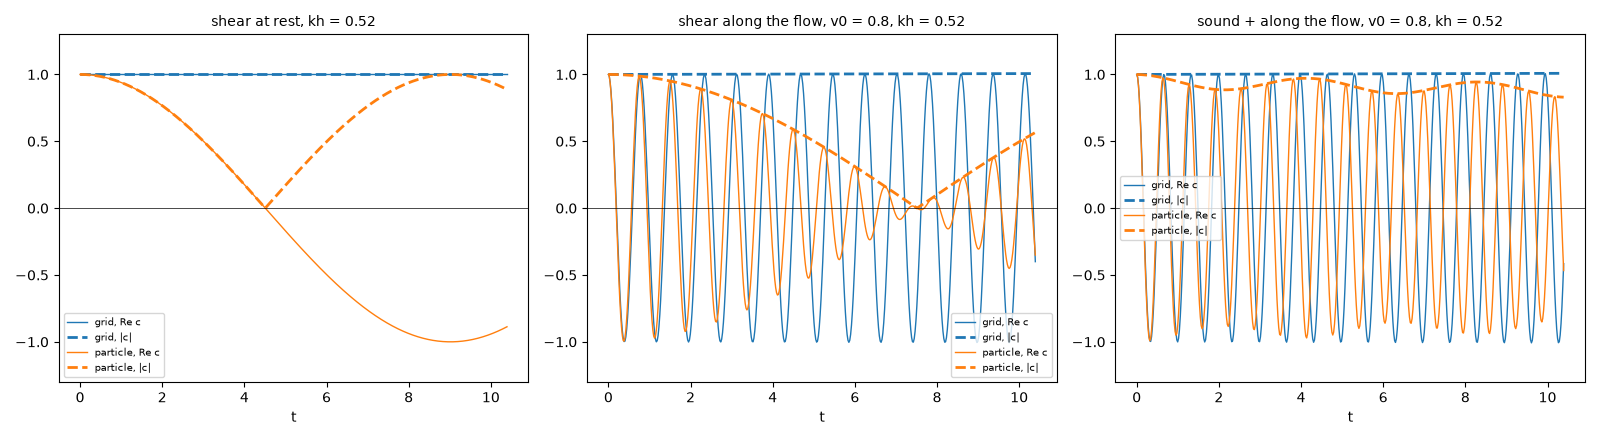
\includegraphics[width=\textwidth]{figs/grid_series.png}
\caption{The mode amplitude $c(t)/|c(0)|$ at $kh=0.52$: real part (thin) and modulus (dashed); blue grid,
orange particles.  Left: shear at rest (the particles oscillate, transverse sound).  Middle: shear
along the flow at $v_0=0.8$ (advected; the particles damp it).  Right: sound $+$ along the flow.}
\label{fig:gseries}
\end{figure}
\begin{figure}[t]
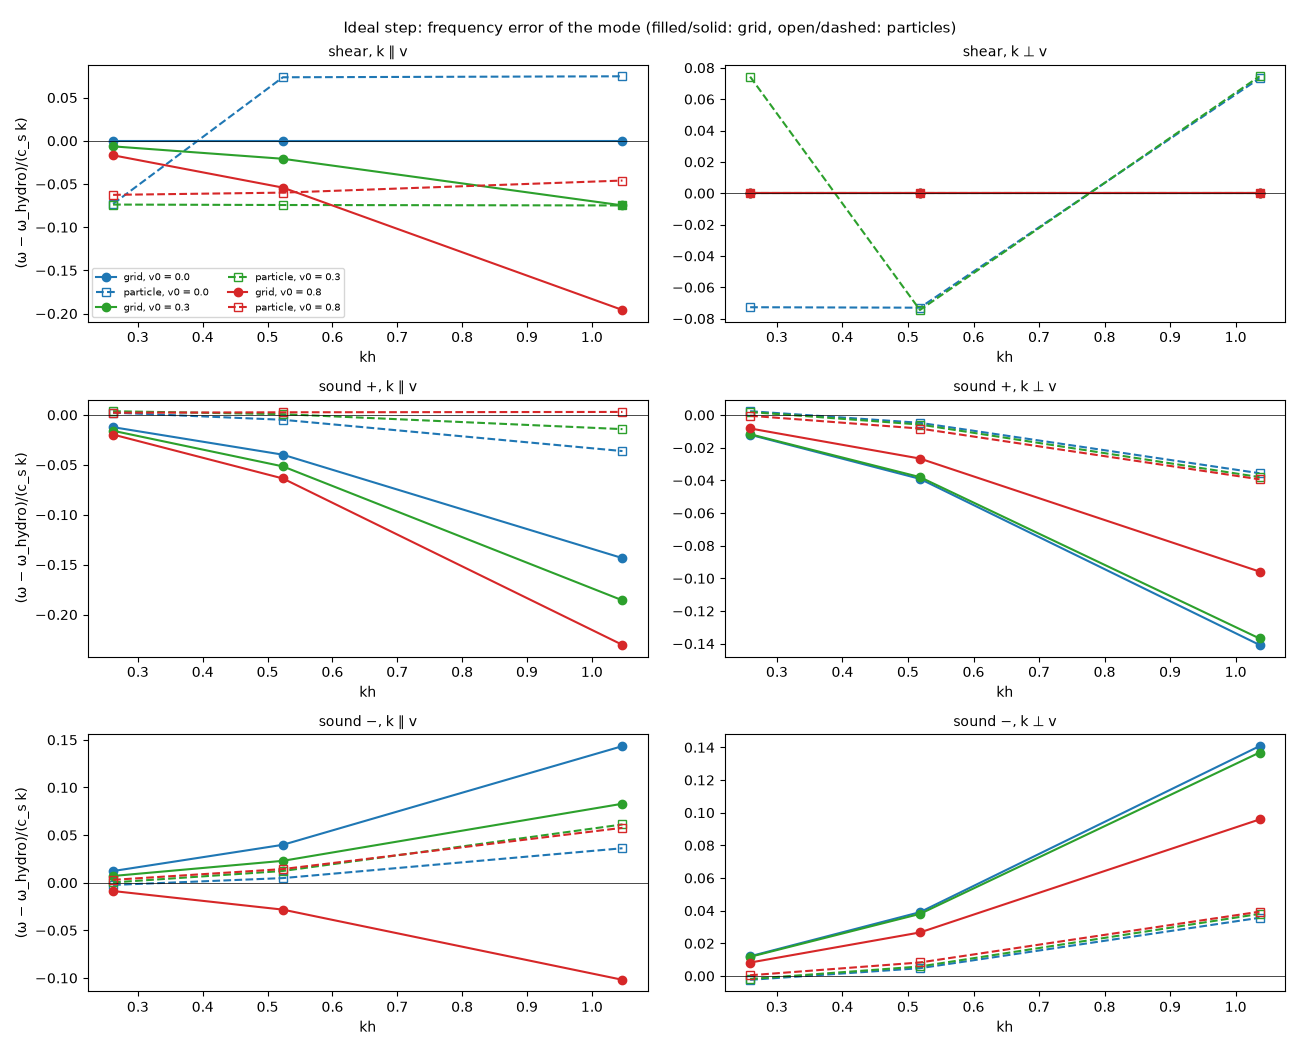
\includegraphics[width=\textwidth]{figs/grid_dispersion.png}
\caption{Frequency error $(\omega-\omega_n)/c_sk$ against $kh$; filled/solid grid, open/dashed particles;
colour $v_0$.  (For the particle shear at rest and across the flow the mode oscillates at $\pm c_tk$
and the sign of the fitted $\omega$ is arbitrary.)}
\label{fig:gdisp}
\end{figure}
\begin{figure}[t]
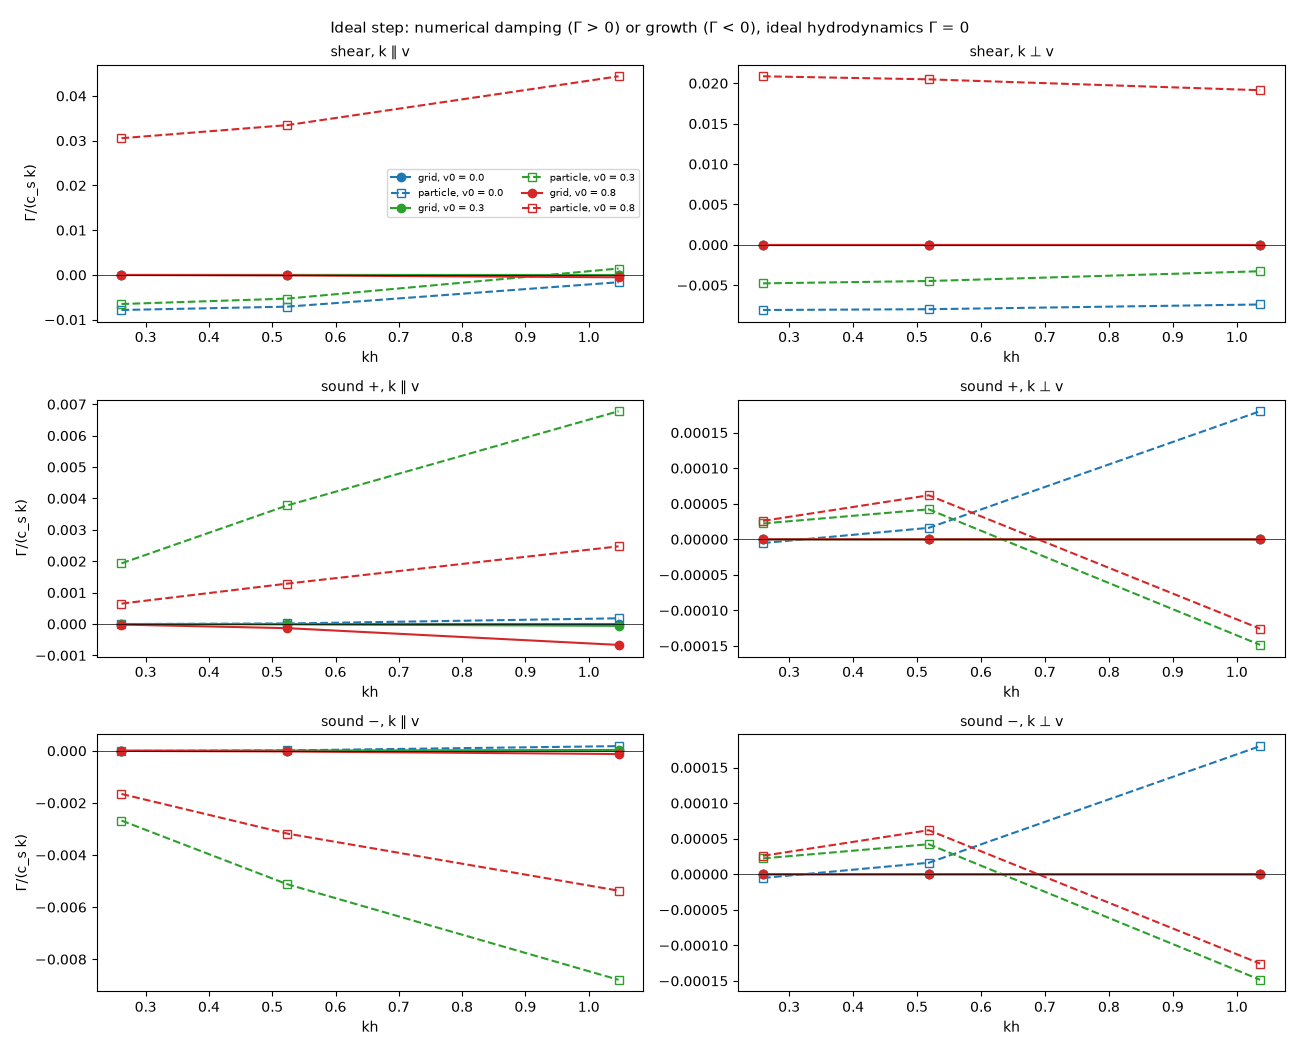
\includegraphics[width=\textwidth]{figs/grid_damping.png}
\caption{Numerical damping $\Gamma/c_sk$ ($\Gamma<0$: growth) of the ideal step against $kh$; as \Fig{fig:gdisp}.
For the particle shear at rest the fit is to an oscillation, not a decay.}
\label{fig:gdamp}
\end{figure}

\begin{figure}[t]
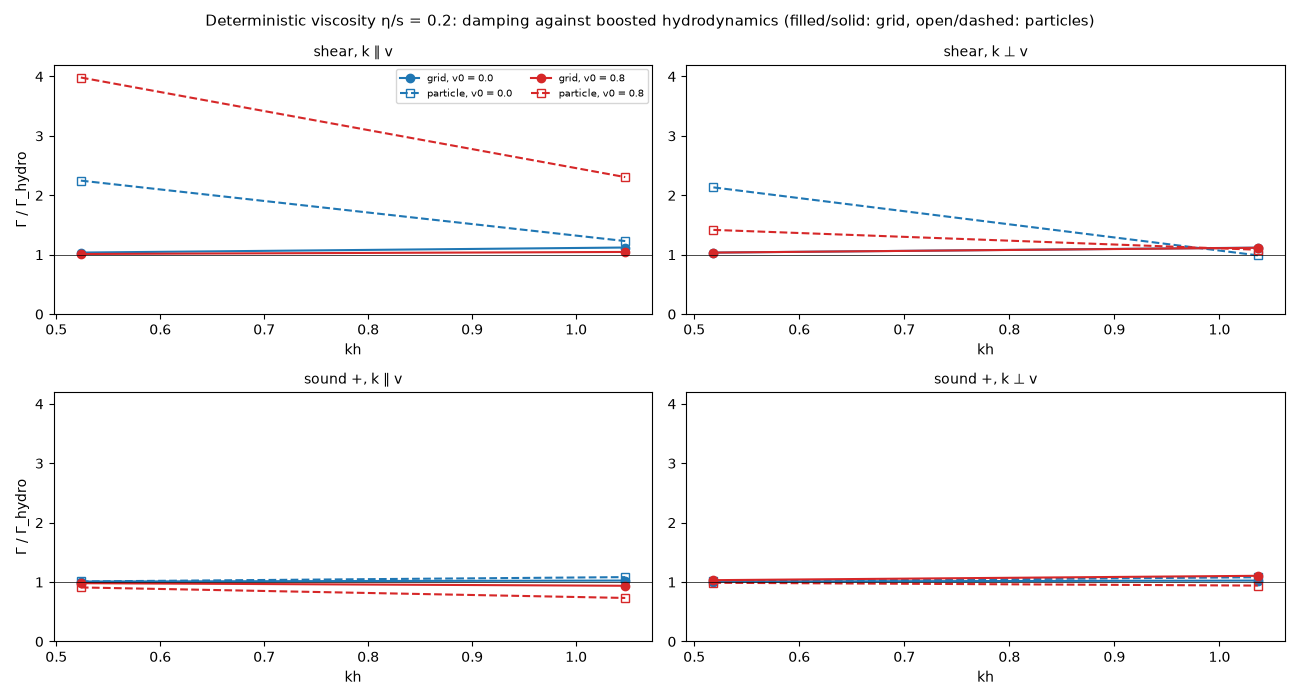
\includegraphics[width=\textwidth]{figs/grid_viscous.png}
\caption{Deterministic viscosity, $\eta/s=0.2$: the fitted damping over boosted hydrodynamics against $kh$,
shear and sound $+$, along and across the flow; filled/solid grid, open/dashed particles; blue $v_0=0$,
red $v_0=0.8$.  (Particle shear at rest: fitted to an oscillation.)}
\label{fig:gvisc}
\end{figure}
\begin{figure}[t]
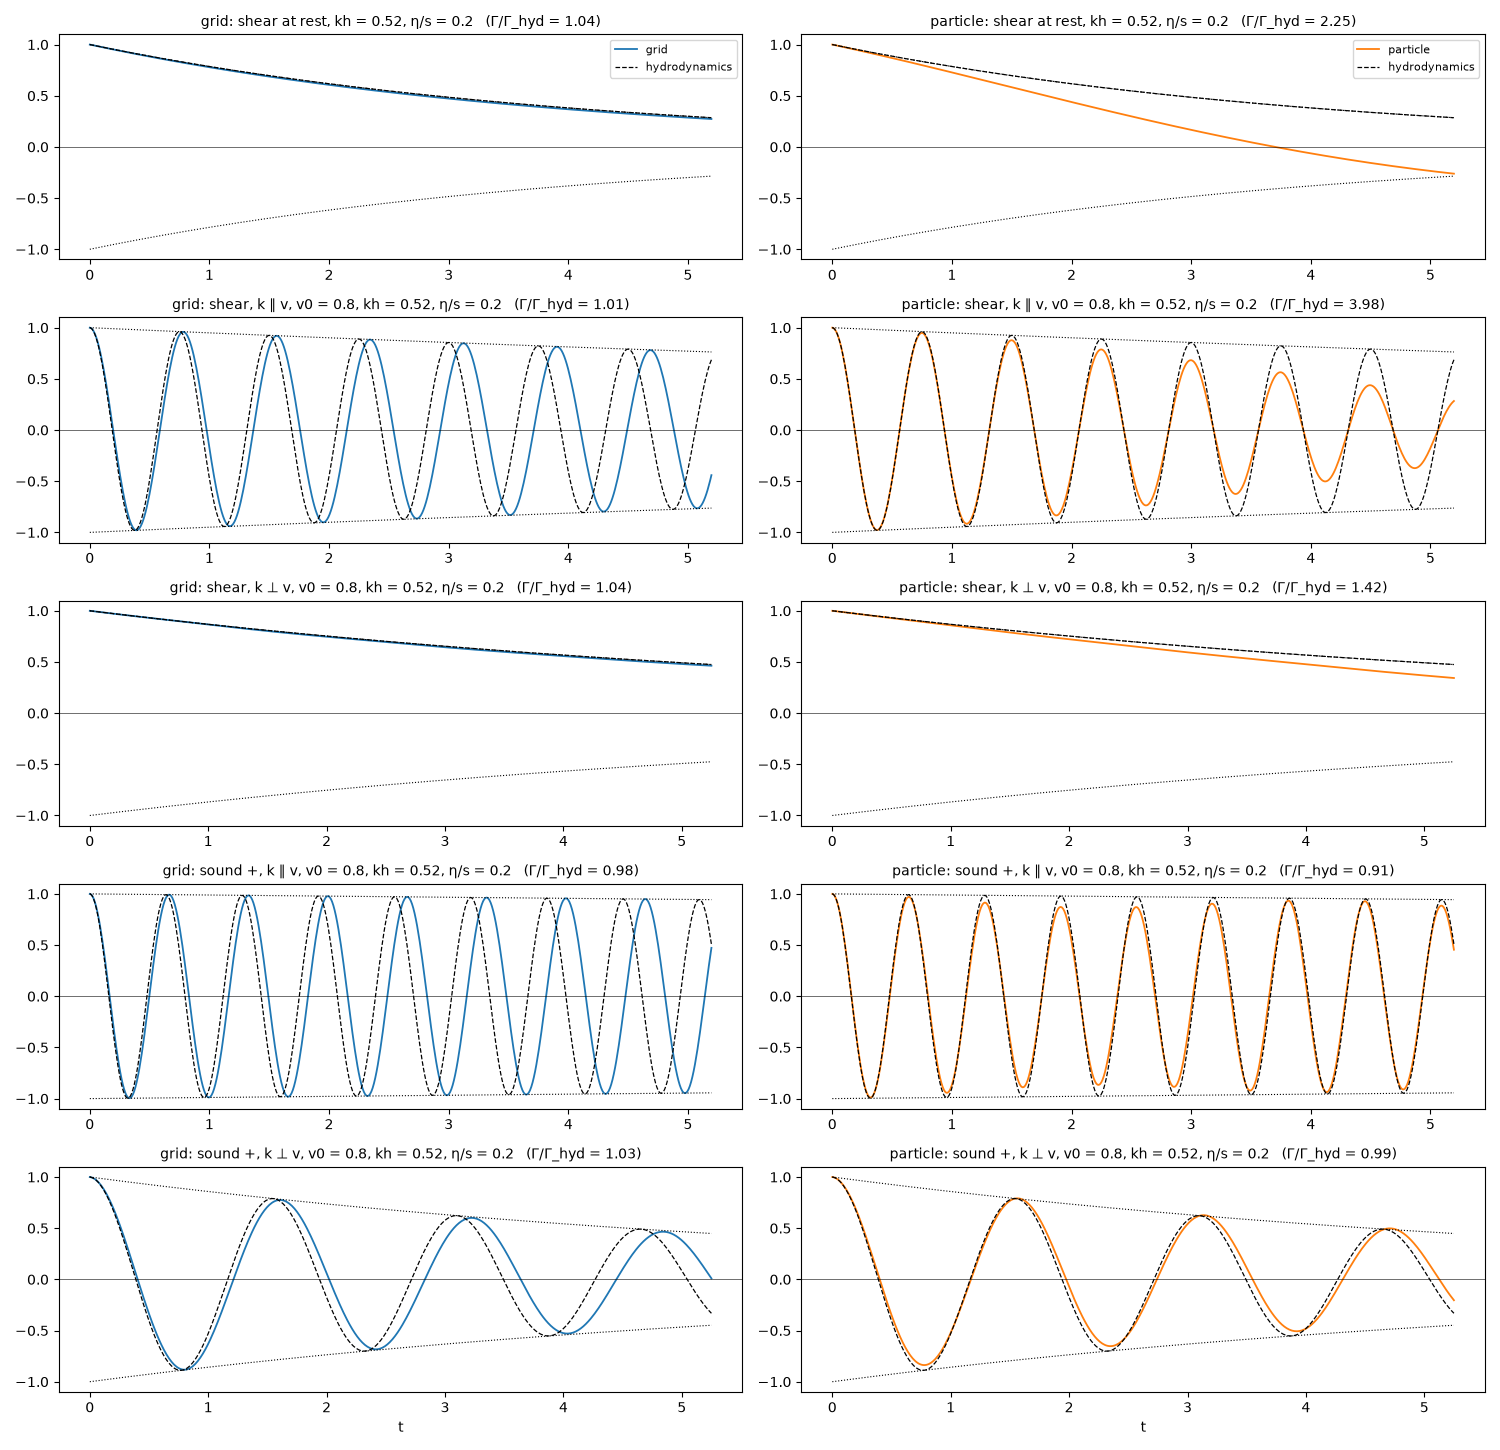
\includegraphics[width=\textwidth]{figs/grid_viscous_series.png}
\caption{Summary of the waves, $\eta/s=0.2$, $kh=0.52$: $\mathrm{Re}\,c(t)/|c(0)|$, grid (left) and particles (right), for the
shear wave at rest, the shear wave along and across the flow at $v_0=0.8$, and sound $+$ along and across
the flow at $v_0=0.8$; dashed boosted hydrodynamics, dotted its envelope.}
\label{fig:gwsum}
\end{figure}
\begin{figure}[p]
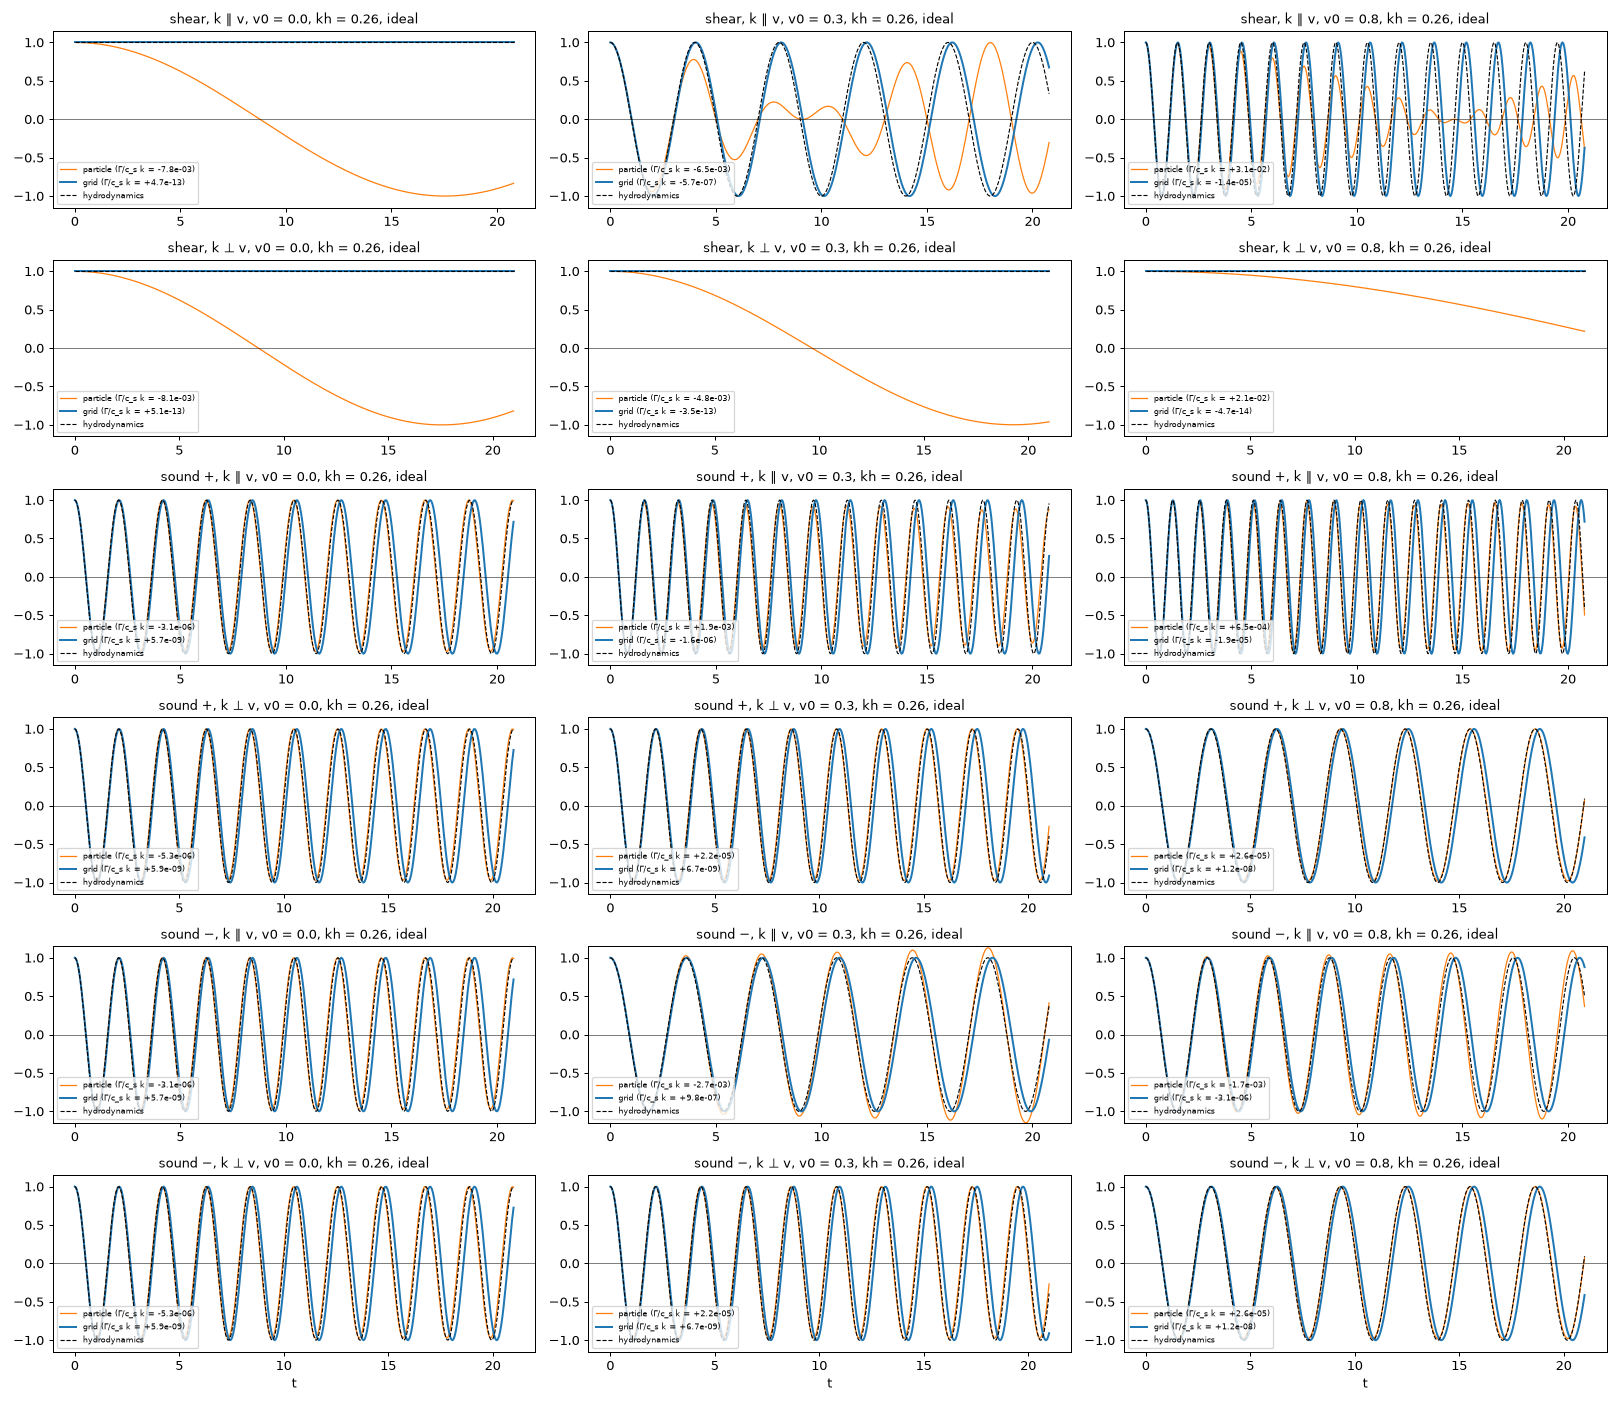
\includegraphics[width=\textwidth]{figs/grid_ideal_waves_kh0.26.png}
\caption{Ideal step, $kh=0.26$: $\mathrm{Re}\,c(t)/|c(0)|$ for each mode (rows: shear, sound $+$, sound $-$; along and across
the flow) and $v_0=0$, $0.3$, $0.8$ (columns); blue grid, orange particles, dashed ideal hydrodynamics; the
legend gives the fitted $\Gamma/c_sk$.}
\label{fig:gw026}
\end{figure}
\begin{figure}[p]
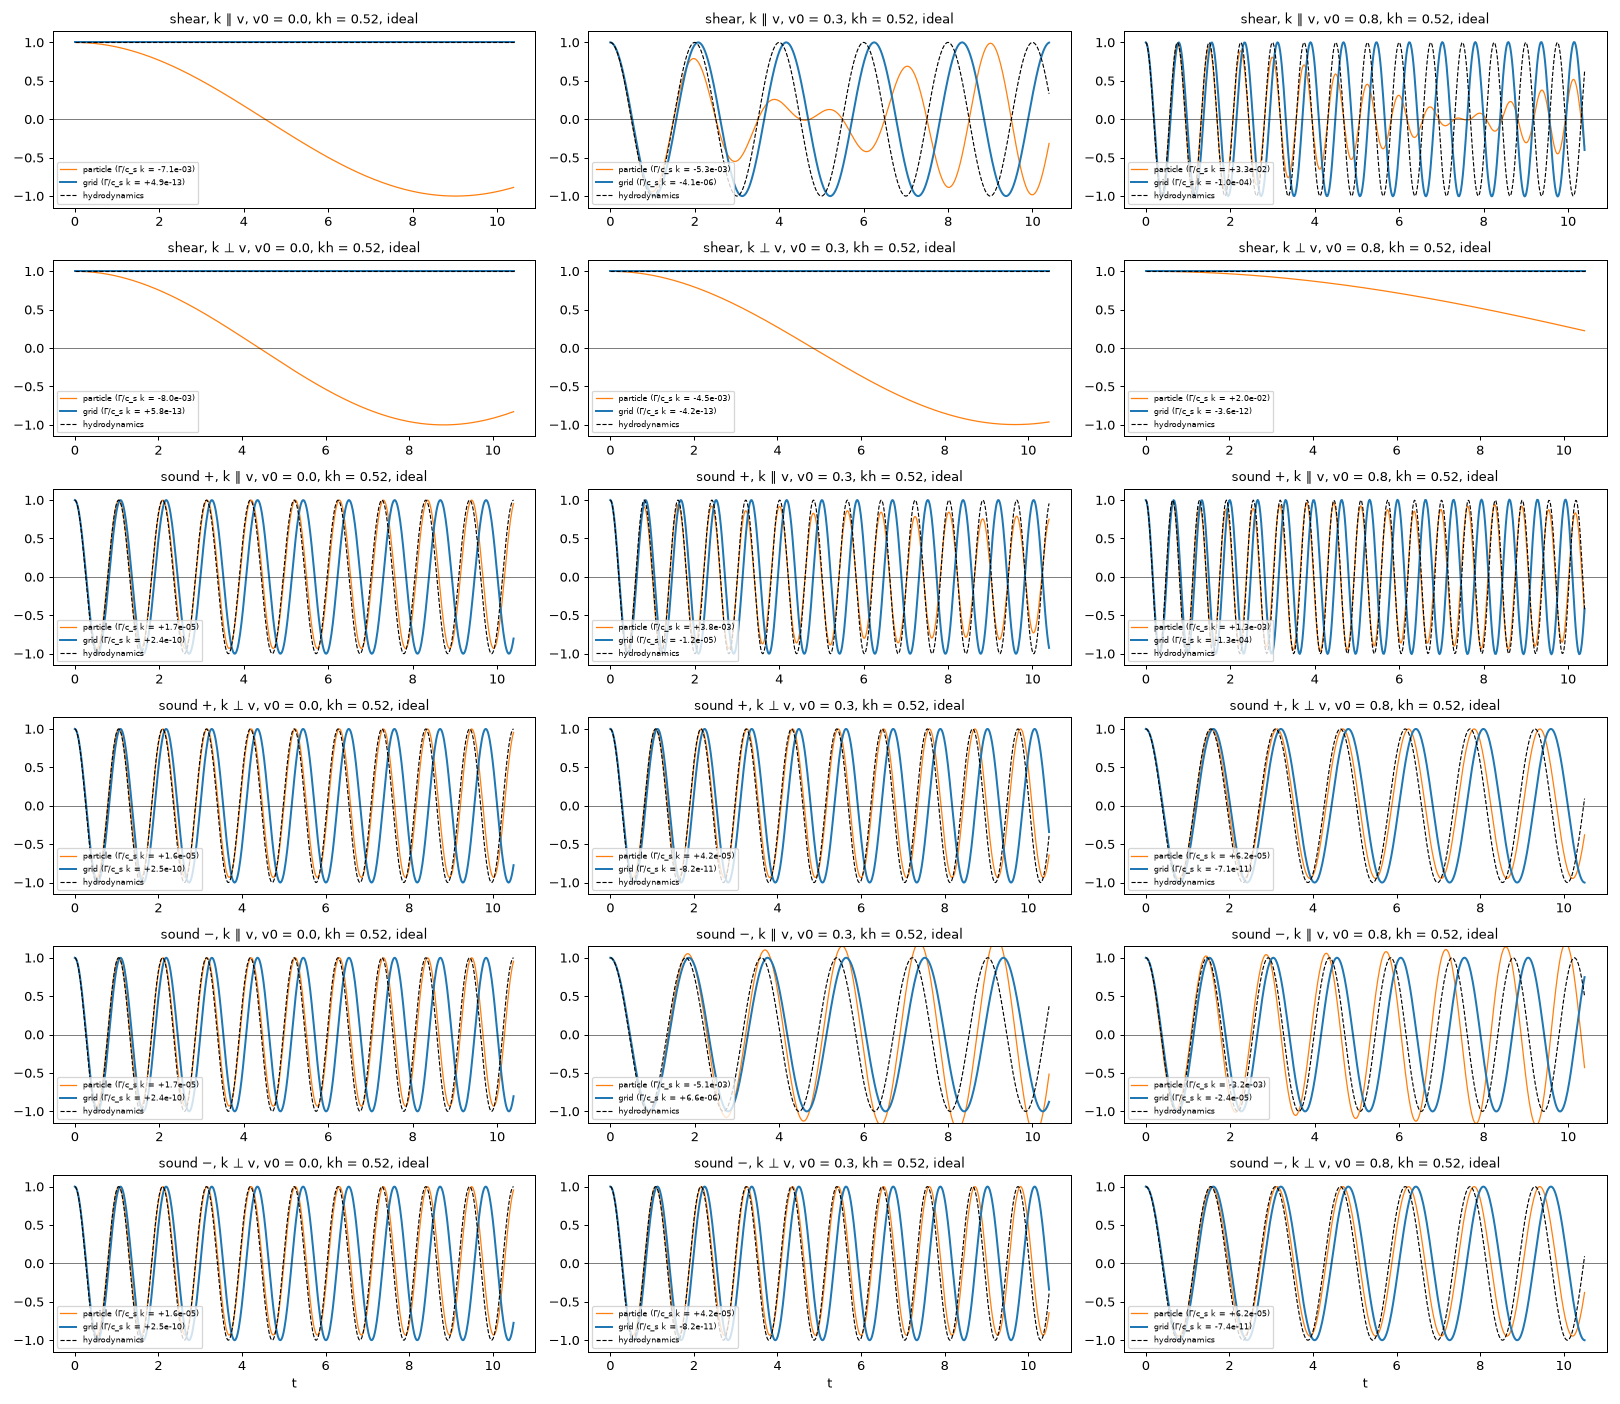
\includegraphics[width=\textwidth]{figs/grid_ideal_waves_kh0.52.png}
\caption{As \Fig{fig:gw026}, $kh=0.52$.}
\label{fig:gw052}
\end{figure}
\begin{figure}[p]
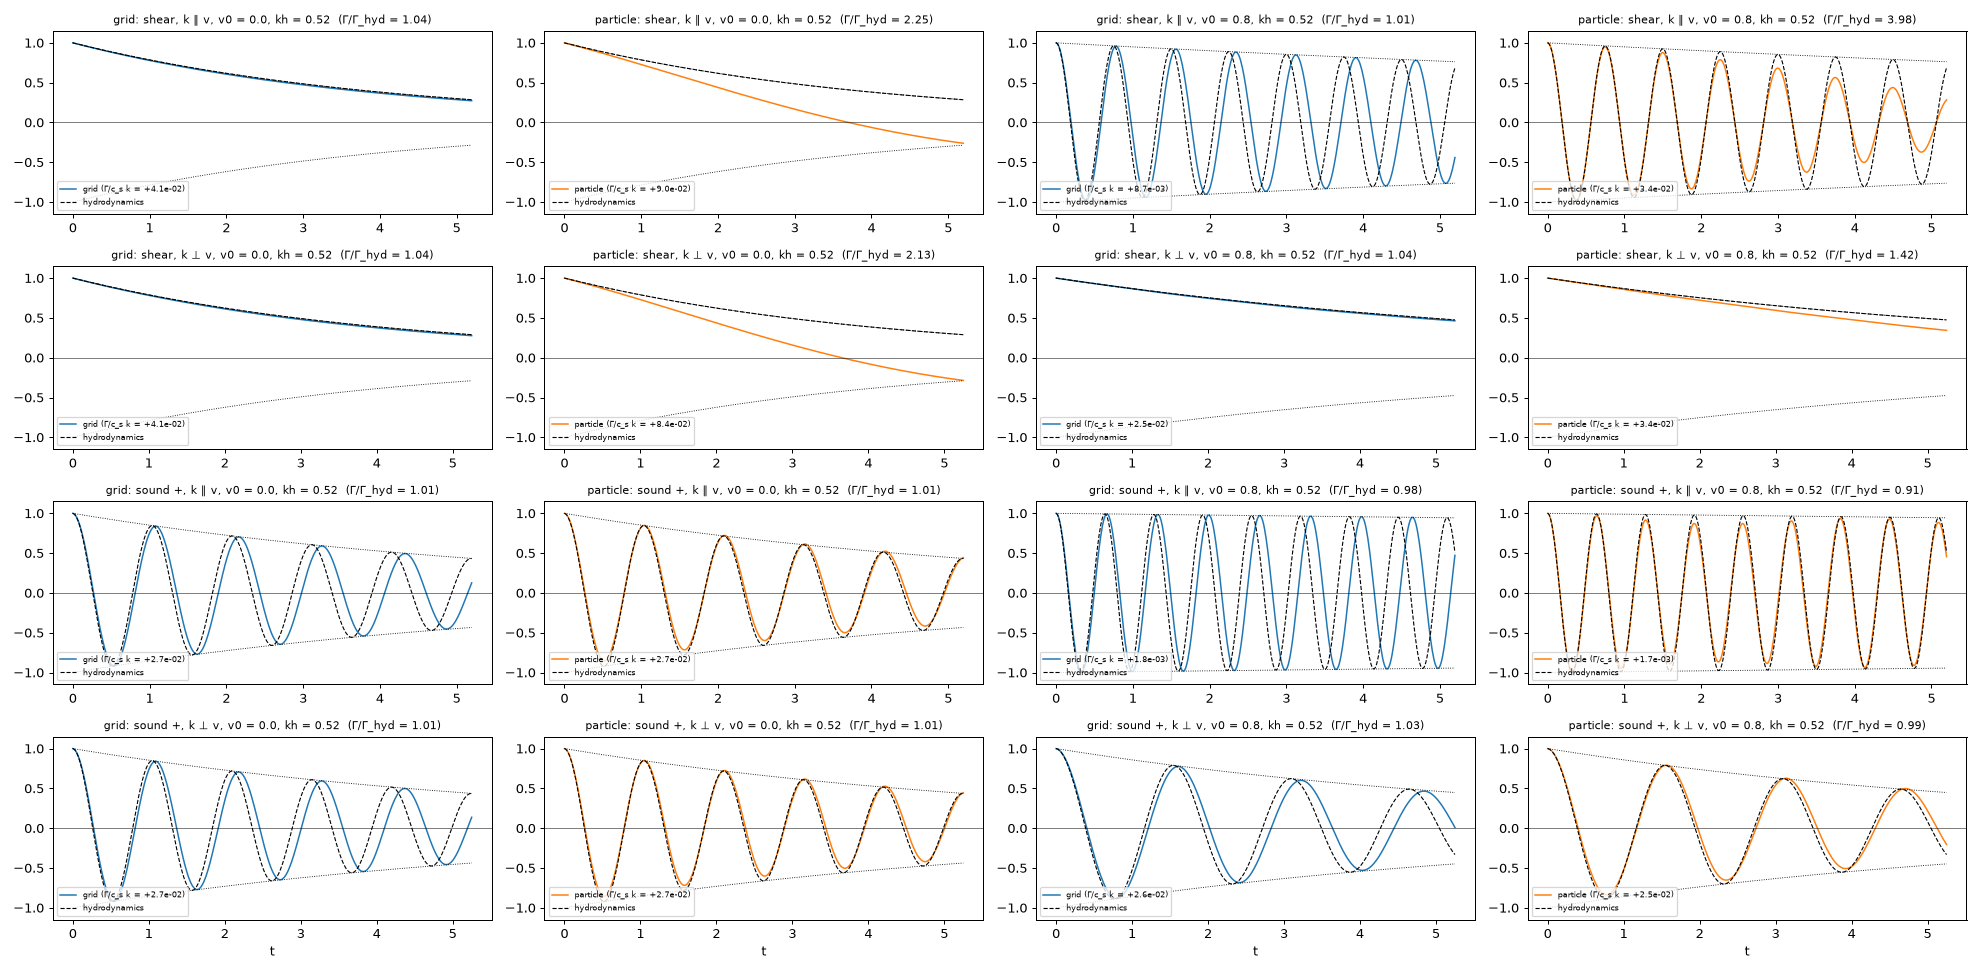
\includegraphics[width=\textwidth]{figs/grid_viscous_waves_kh0.52.png}
\caption{Deterministic viscosity $\eta/s=0.2$, $kh=0.52$: shear and sound $+$, along and across the flow (rows);
columns: grid and particles at $v_0=0$, grid and particles at $v_0=0.8$; dashed boosted hydrodynamics,
dotted its envelope.}
\label{fig:gwv052}
\end{figure}
\begin{figure}[p]
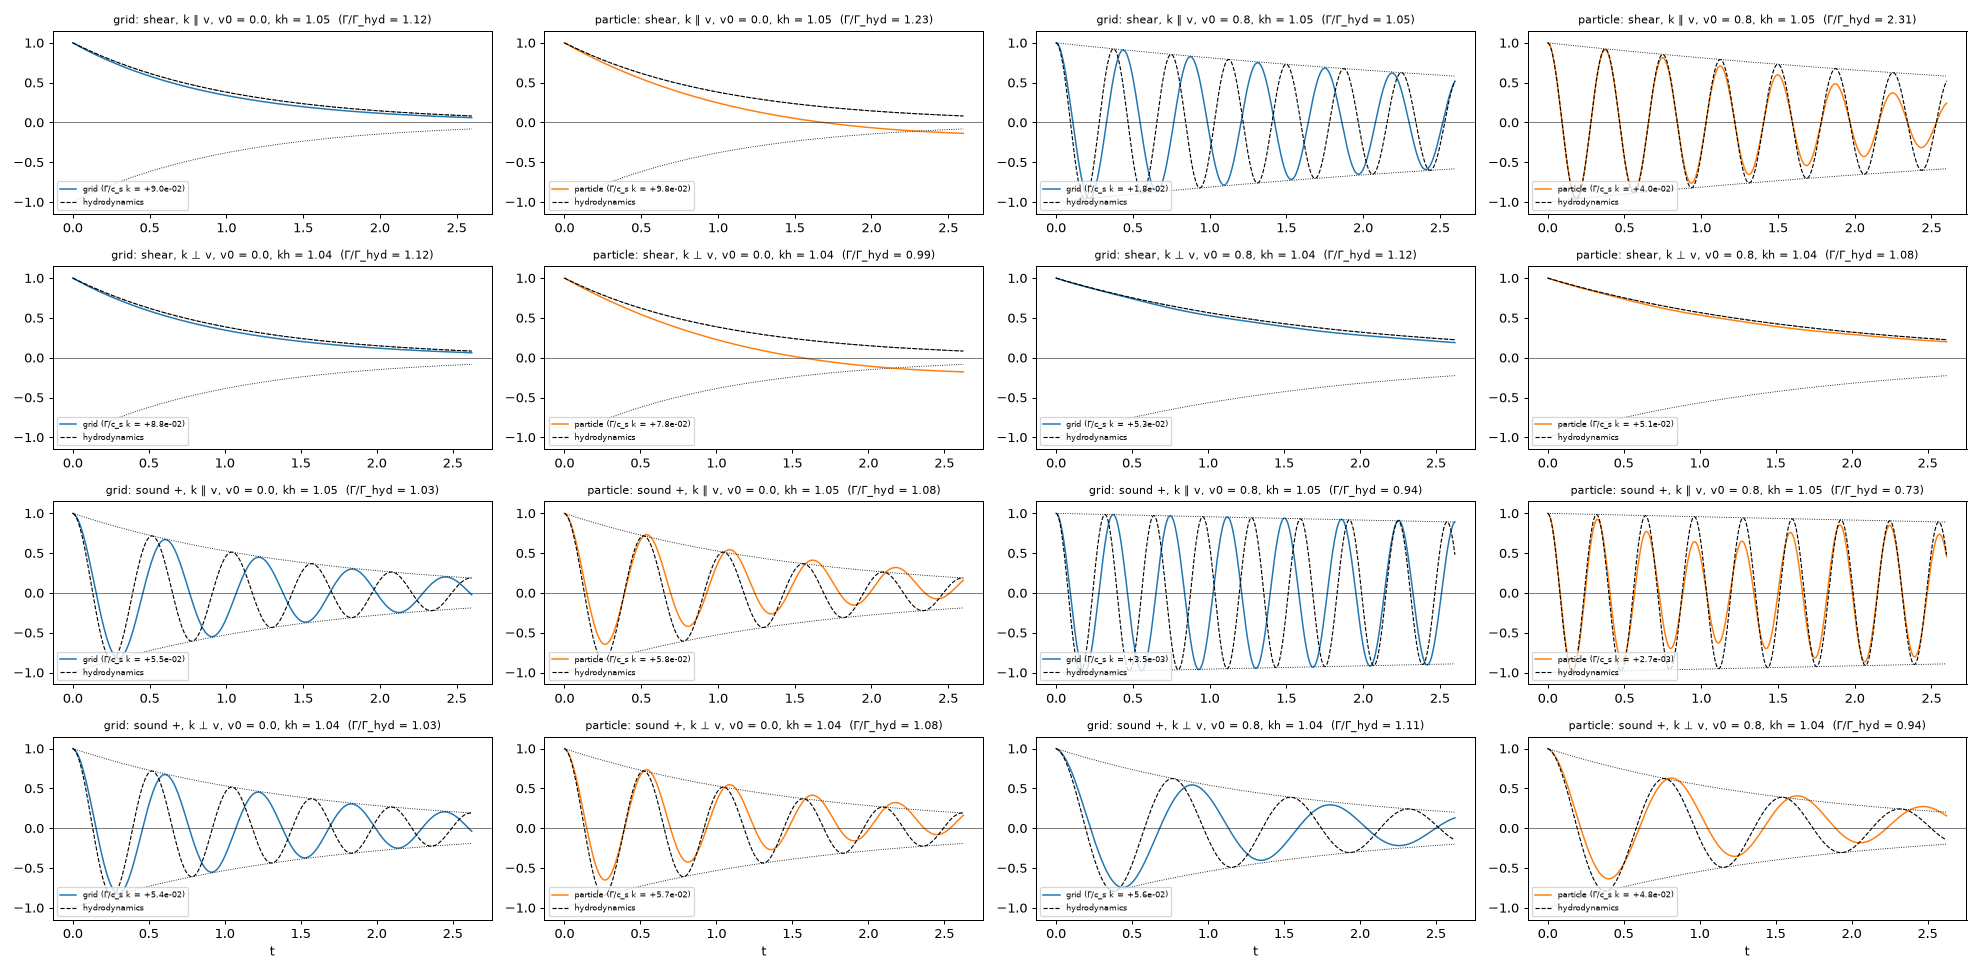
\includegraphics[width=\textwidth]{figs/grid_viscous_waves_kh1.05.png}
\caption{As \Fig{fig:gwv052}, $kh=1.05$.}
\label{fig:gwv105}
\end{figure}
\begin{figure}[t]
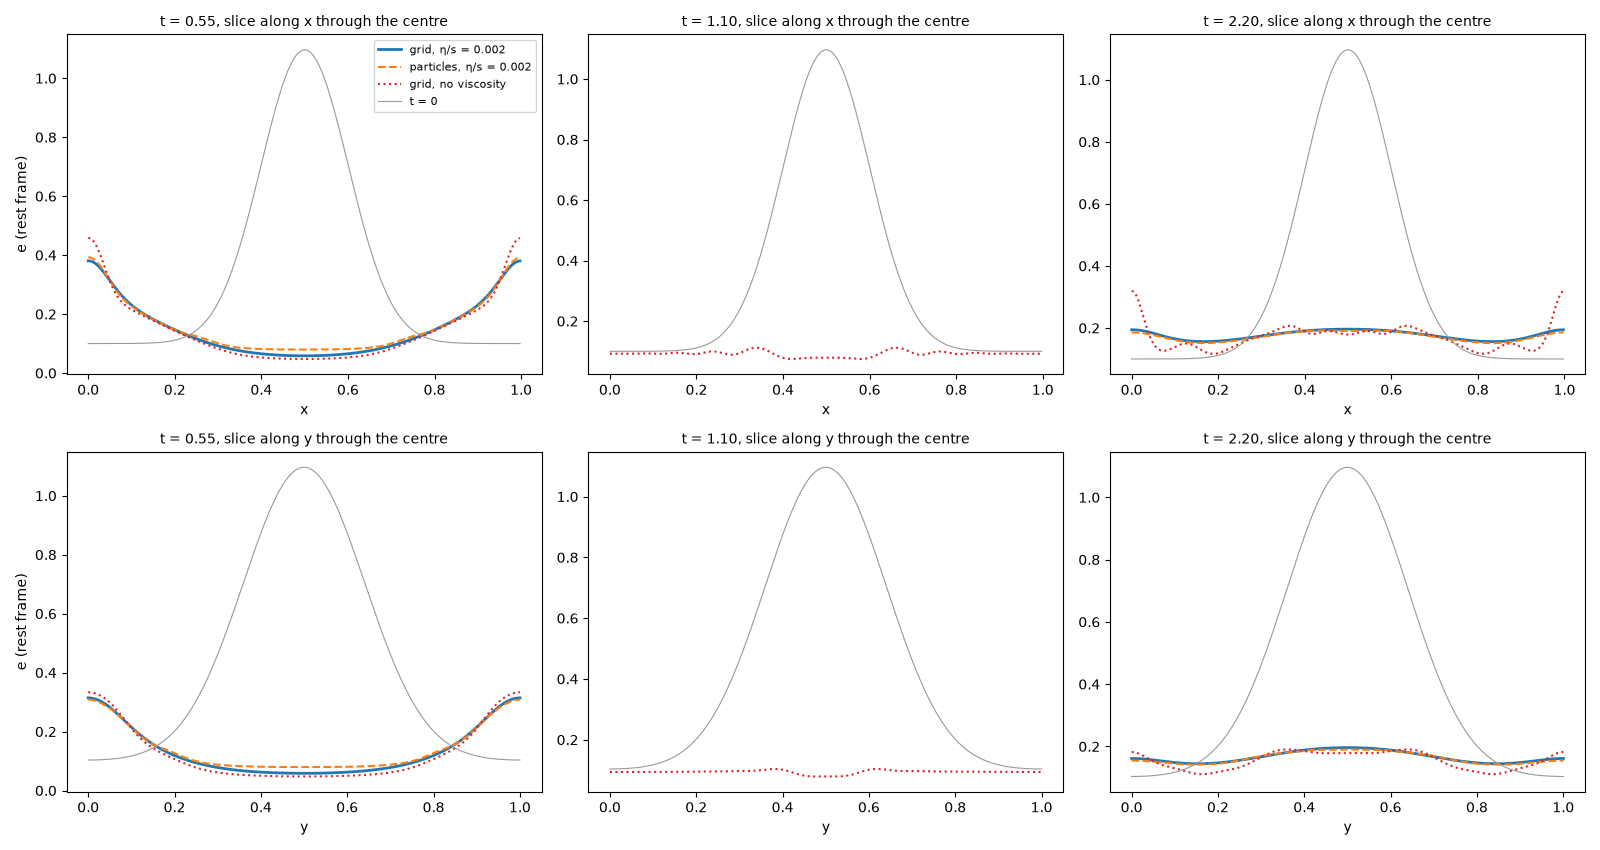
\includegraphics[width=\textwidth]{figs/grid_gaussian_slices.png}
\caption{Gaussian pulse: the rest-frame energy density along $x$ (top) and $y$ (bottom) through the
centre at $t=0.55$, $1.1$, $2.2$; grid with $\eta/s=0.002$ (blue), particles with $\eta/s=0.002$ (orange),
grid without viscosity (red).  At $t=0$ the pulse is $0.1+e^{-x^2/2\sigma_x^2-y^2/2\sigma_y^2}$ (peak $1.1$).  The
$t=1.1$ profiles of the two viscous runs are missing.}
\label{fig:ggslice}
\end{figure}
\begin{figure}[t]
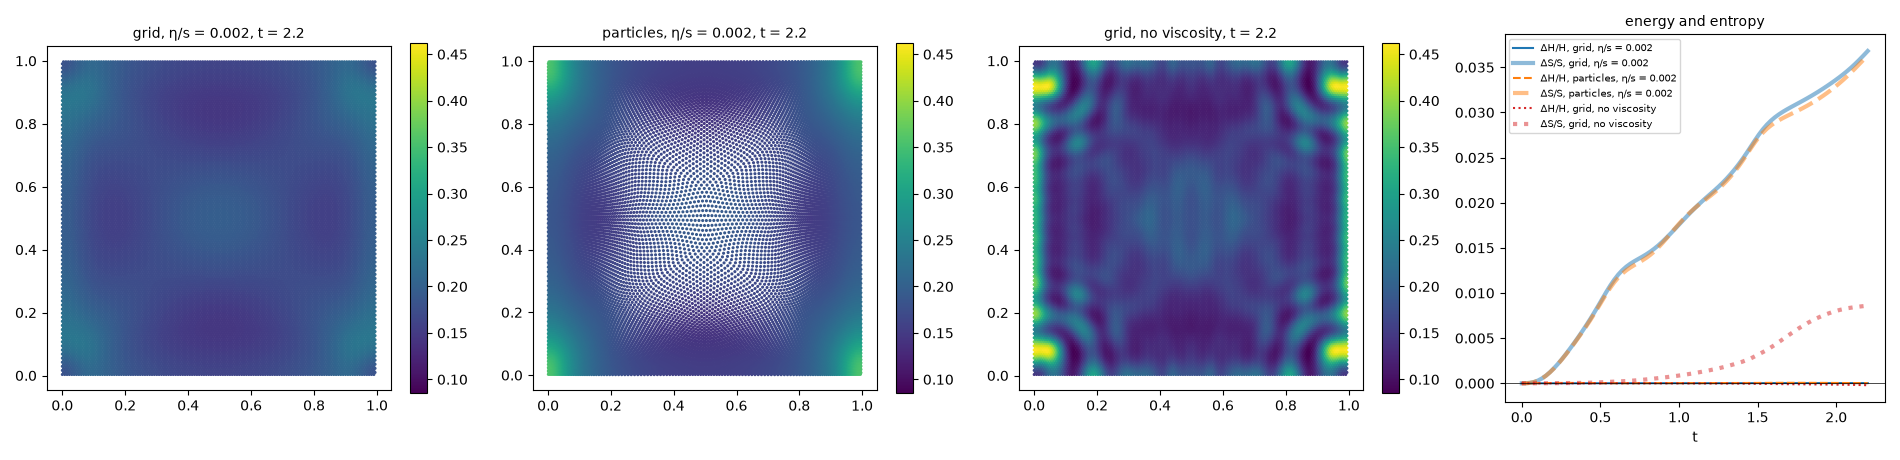
\includegraphics[width=\textwidth]{figs/grid_gaussian_maps.png}
\caption{Gaussian pulse at $t=2.2$: the energy density on the sites (grid) and on the particles (which
have moved), and $\Delta H/H$, $\Delta S/S$ against $t$.}
\label{fig:ggmap}
\end{figure}
\begin{figure}[p]
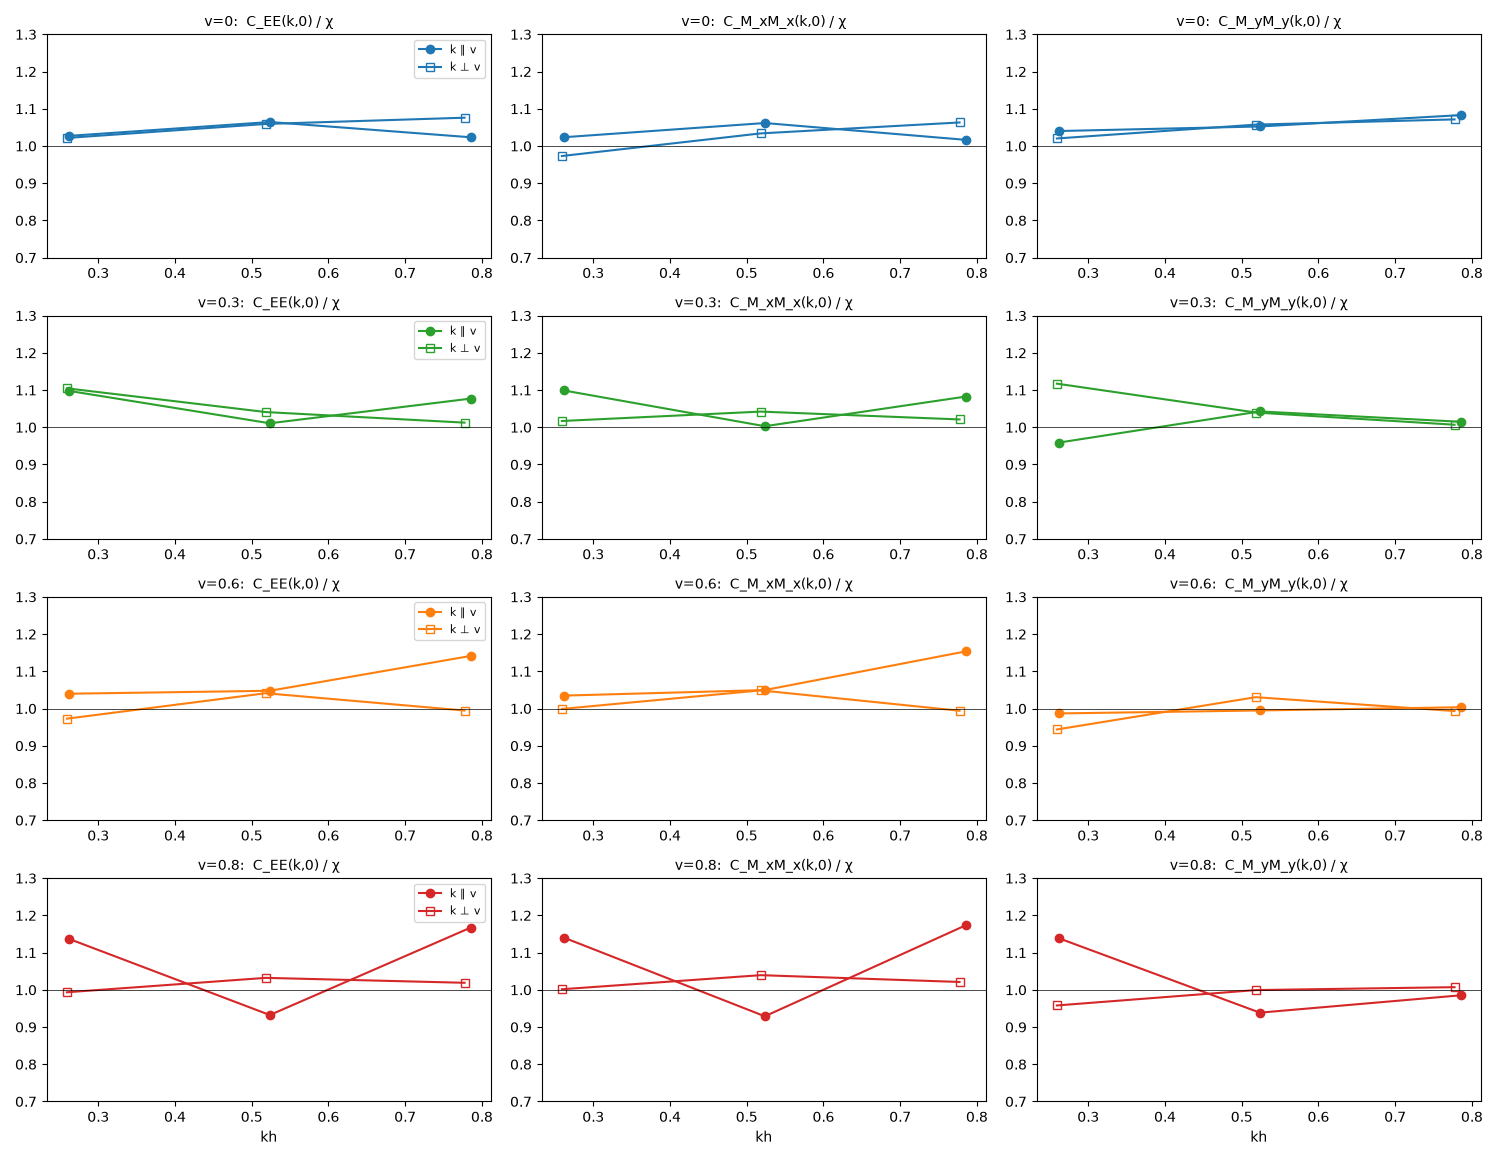
\includegraphics[width=\textwidth]{figs/boost_static_GRID.png}
\caption{Stochastic grid campaign: equal-time $C_{AA}(\bm k,0)/\chi_{AA}$ against $kh$, one row per $v_0$ (as \texttt{boost.tex}, Fig.~1);
filled $\bm k\parallel\bm v$, open $\bm k\perp\bm v$.}
\label{fig:gbstatic}
\end{figure}
\begin{figure}[p]
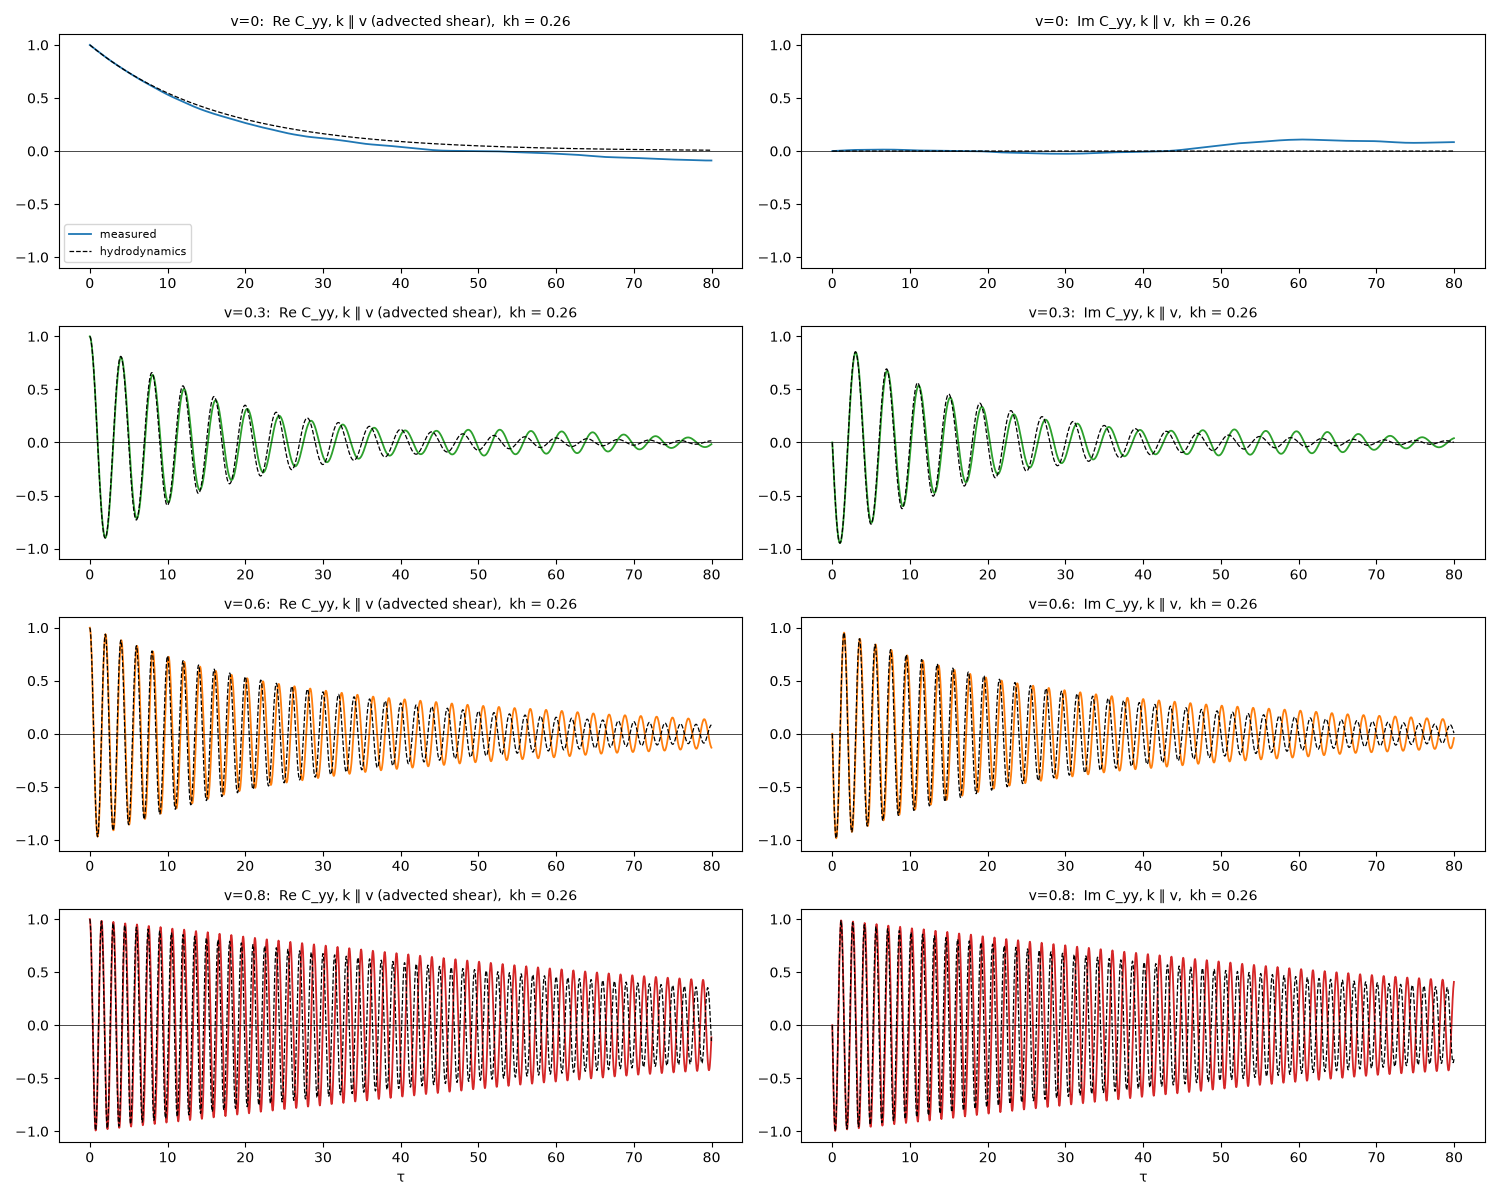
\includegraphics[width=\textwidth]{figs/boost_shear_GRID.png}
\caption{Stochastic grid campaign: the advected shear mode, $C_{yy}(k\hat x,\tau)/C_{yy}(k\hat x,0)$ at $kh=0.26$, one row per $v_0$;
dashed hydrodynamics.}
\label{fig:gbshear}
\end{figure}
\begin{figure}[p]
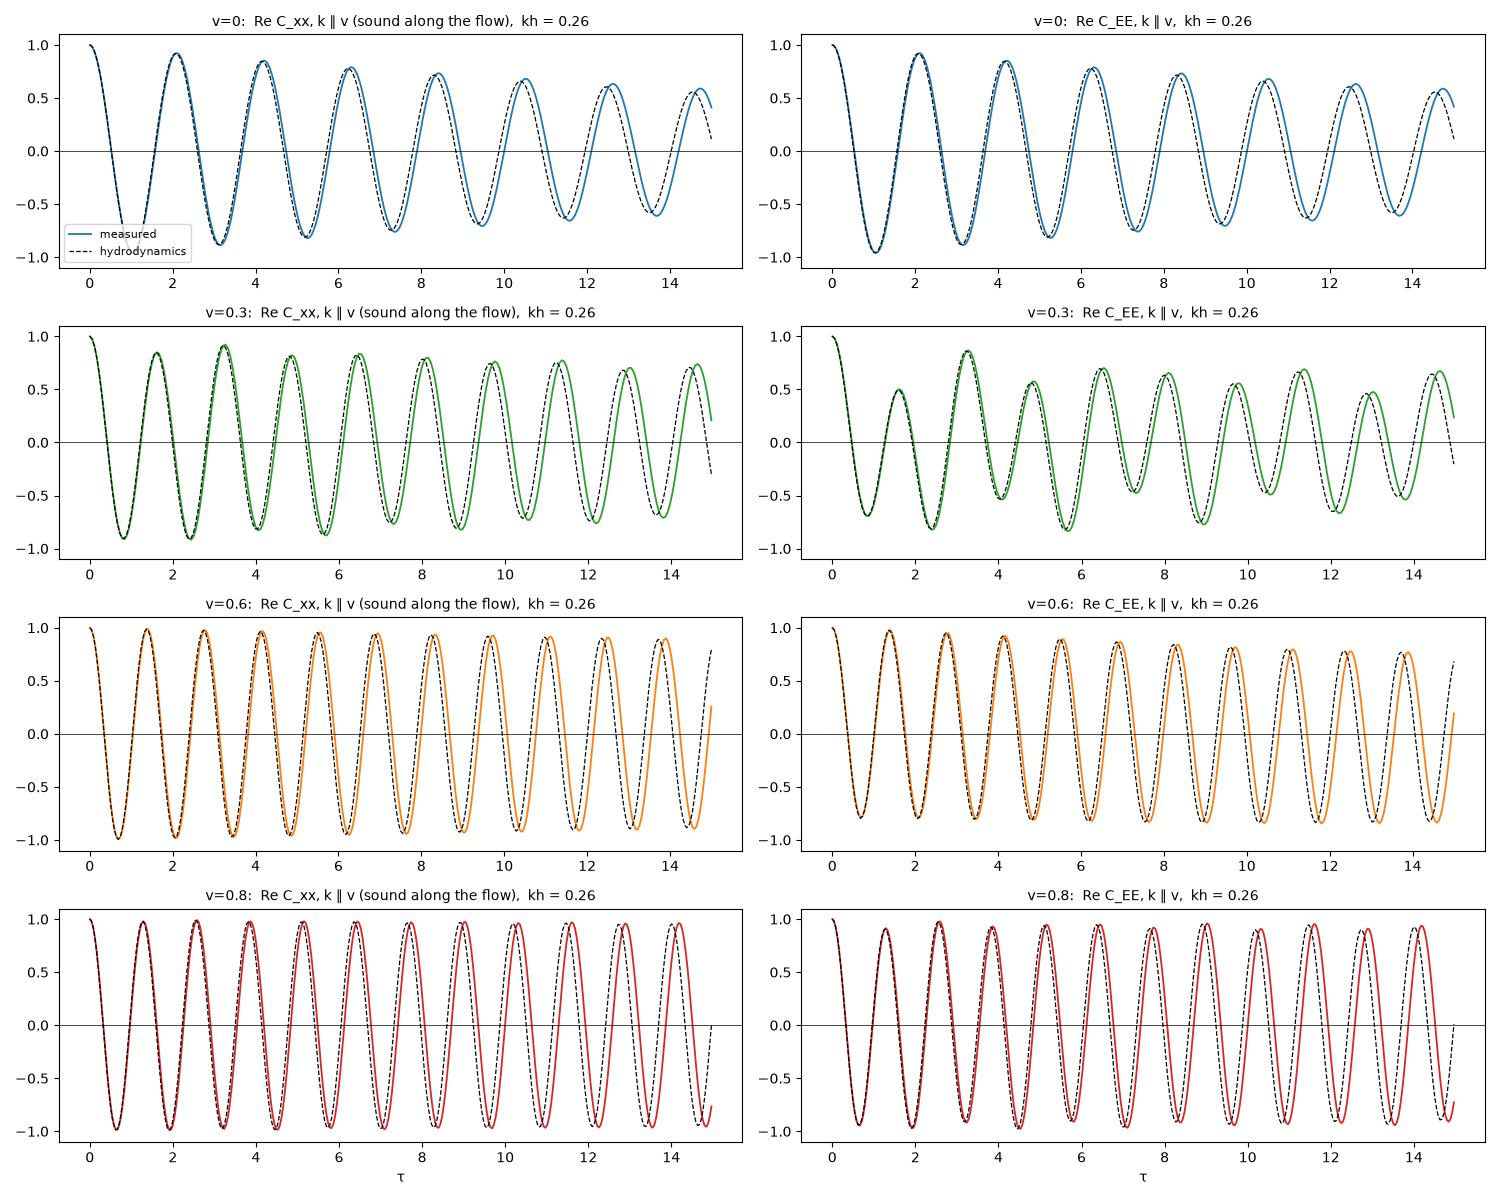
\includegraphics[width=\textwidth]{figs/boost_par_GRID.png}
\caption{Stochastic grid campaign: sound along the flow, $\mathrm{Re}\,C_{xx}$ and $\mathrm{Re}\,C_{EE}$ for $\bm k\parallel\bm v$ at $kh=0.26$, one row per $v_0$;
dashed hydrodynamics (as \texttt{boost.tex}, Fig.~3).}
\label{fig:gbpar}
\end{figure}
\begin{figure}[p]
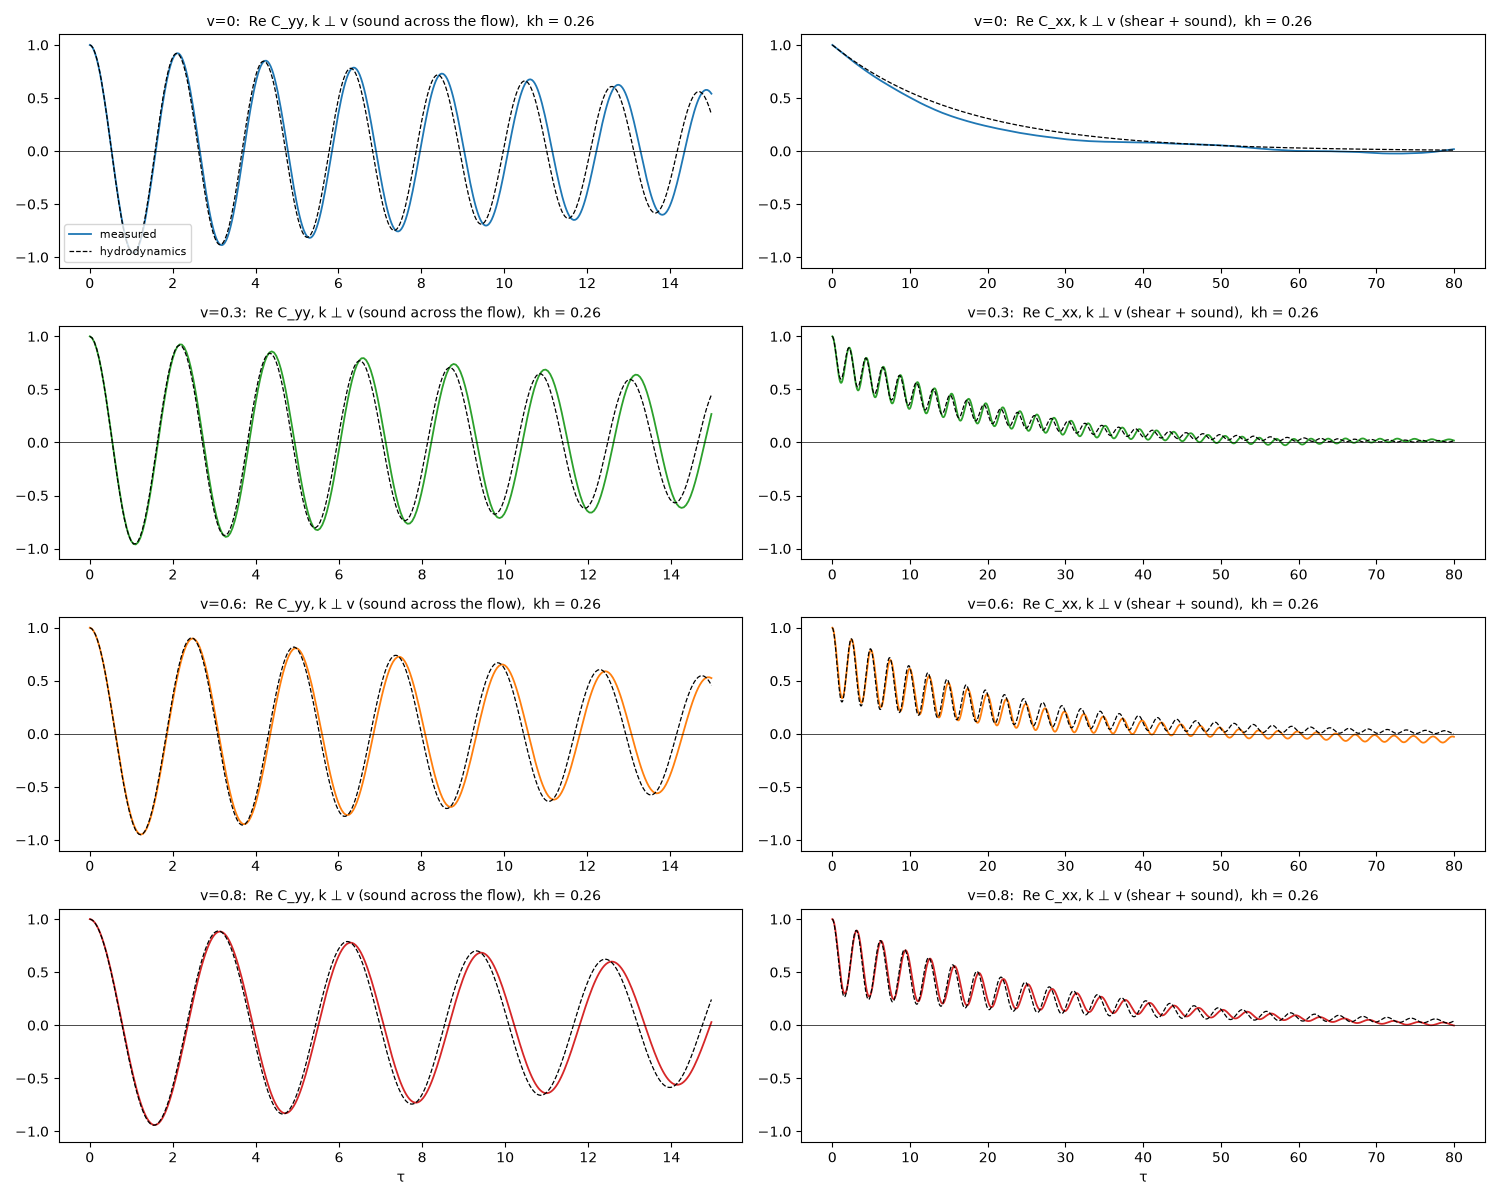
\includegraphics[width=\textwidth]{figs/boost_perp_GRID.png}
\caption{Stochastic grid campaign: across the flow, $\mathrm{Re}\,C_{yy}$ (sound) and $\mathrm{Re}\,C_{xx}$ (shear mixed with sound) for $\bm k\perp\bm v$
at $kh=0.26$, one row per $v_0$ (as \texttt{boost.tex}, Fig.~4).}
\label{fig:gbperp}
\end{figure}
\begin{figure}[t]
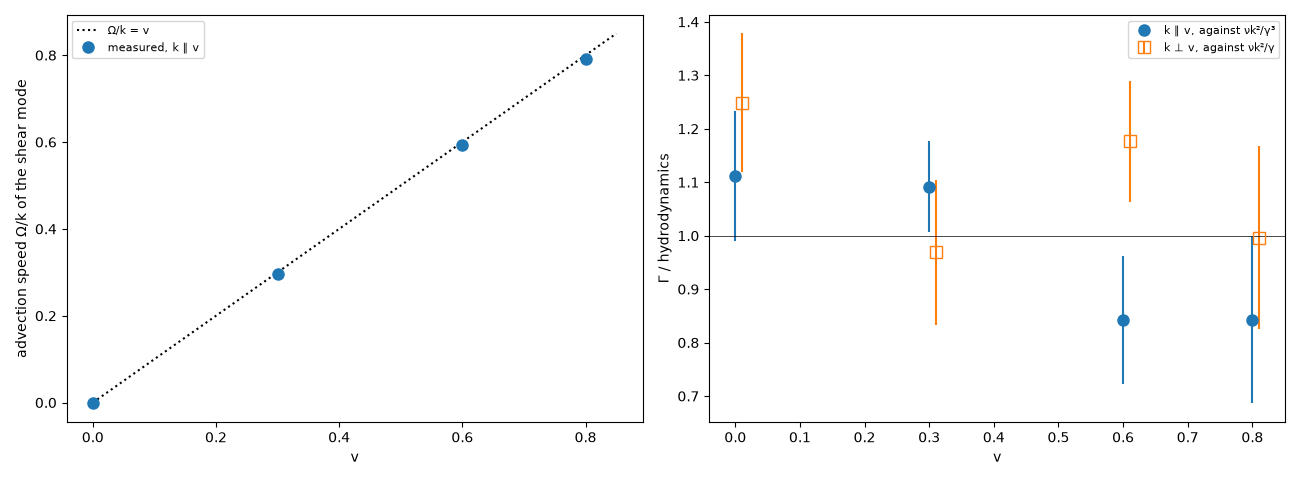
\includegraphics[width=\textwidth]{figs/boost_fit_GRID.png}
\caption{Stochastic grid campaign: fitted advection speed and shear damping against $v_0$ at $kh=0.26$ (as \texttt{boost.tex}, Fig.~5).}
\label{fig:gbfit}
\end{figure}
\begin{figure}[t]
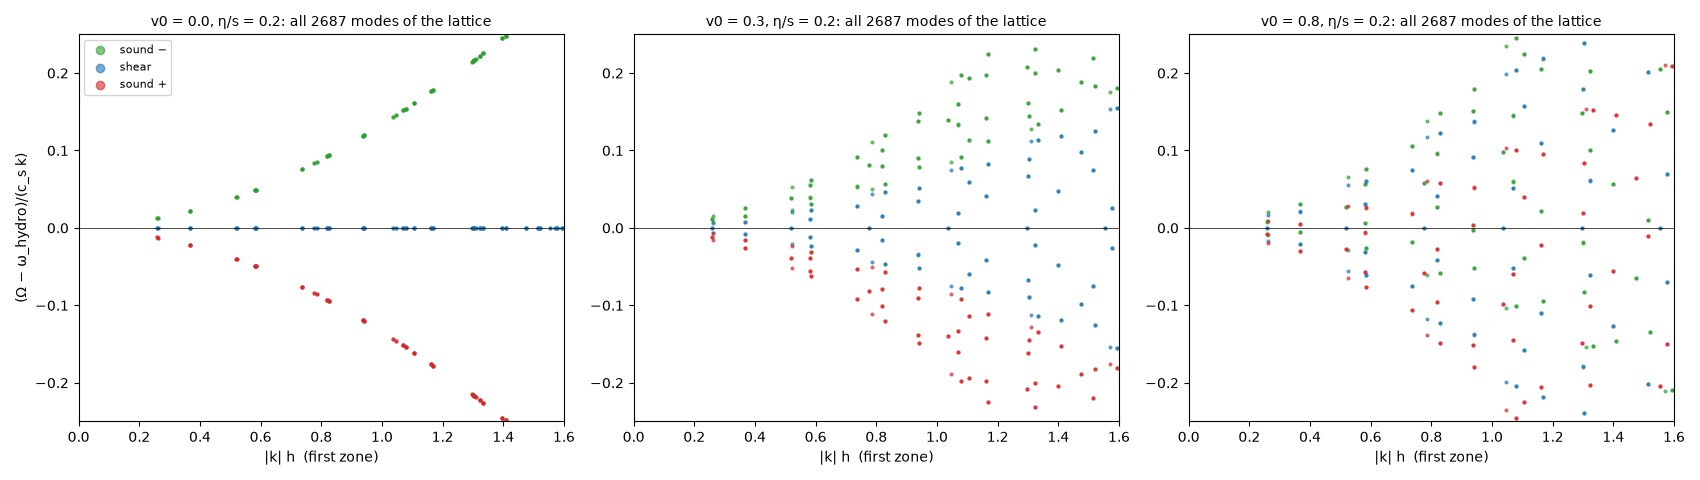
\includegraphics[width=\textwidth]{figs/grid_bare_freq.png}
\caption{Bare lattice propagator, $\eta/s=0.2$: the frequency error $(\Omega-\omega_{\rm hydro})/c_sk$ of every mode of the lattice
against $|\bm k|h$ (first zone), in the hydrodynamic range; colour: the three modes, sorted by $\Omega$.}
\label{fig:gbfreq}
\end{figure}
\begin{figure}[t]
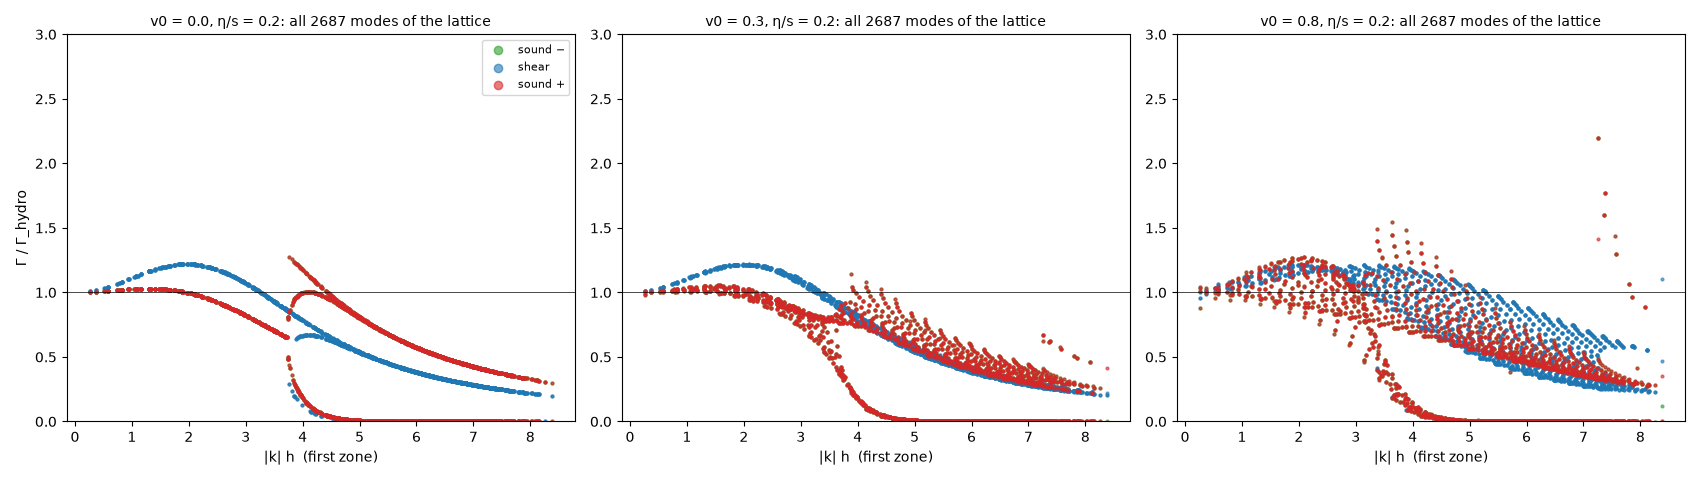
\includegraphics[width=\textwidth]{figs/grid_bare_damp.png}
\caption{Bare lattice propagator, $\eta/s=0.2$: $\Gamma/\Gamma_{\rm hydro}$ of every mode over the whole zone, $v_0=0$, $0.3$, $0.8$.}
\label{fig:gbdamp}
\end{figure}
\begin{figure}[t]
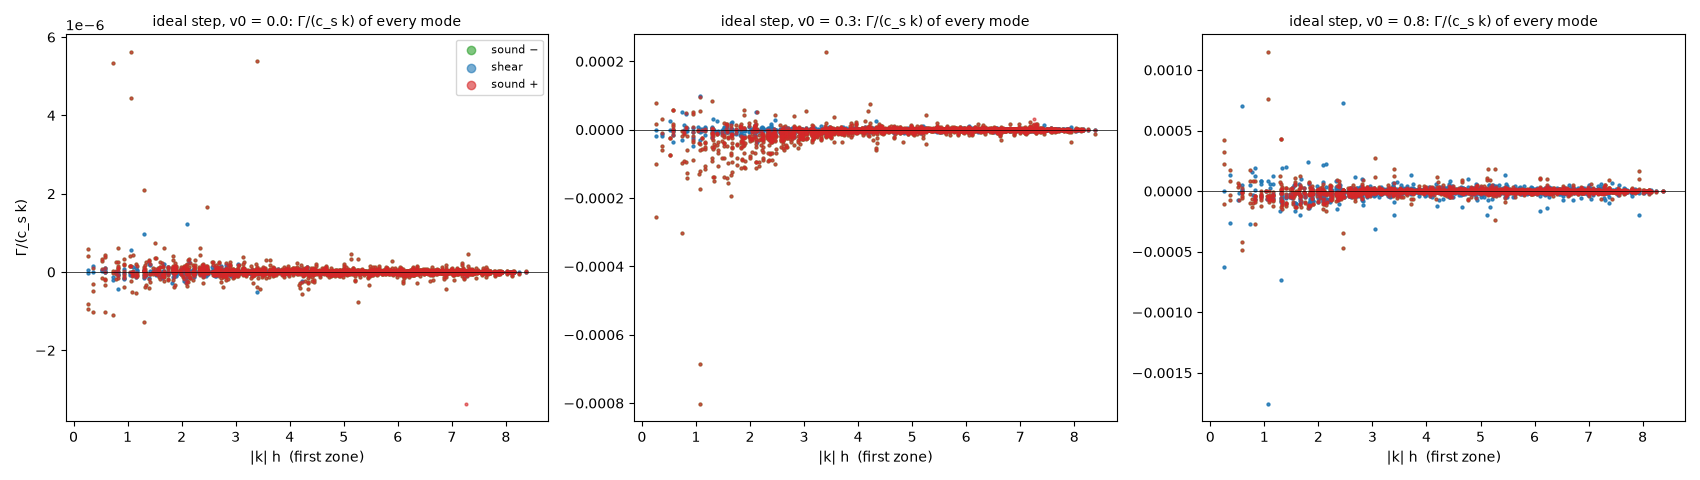
\includegraphics[width=\textwidth]{figs/grid_bare_ideal.png}
\caption{Bare lattice propagator of the ideal step: $\Gamma/c_sk$ of every mode (note the scales).}
\label{fig:gbideal}
\end{figure}
\begin{figure}[t]
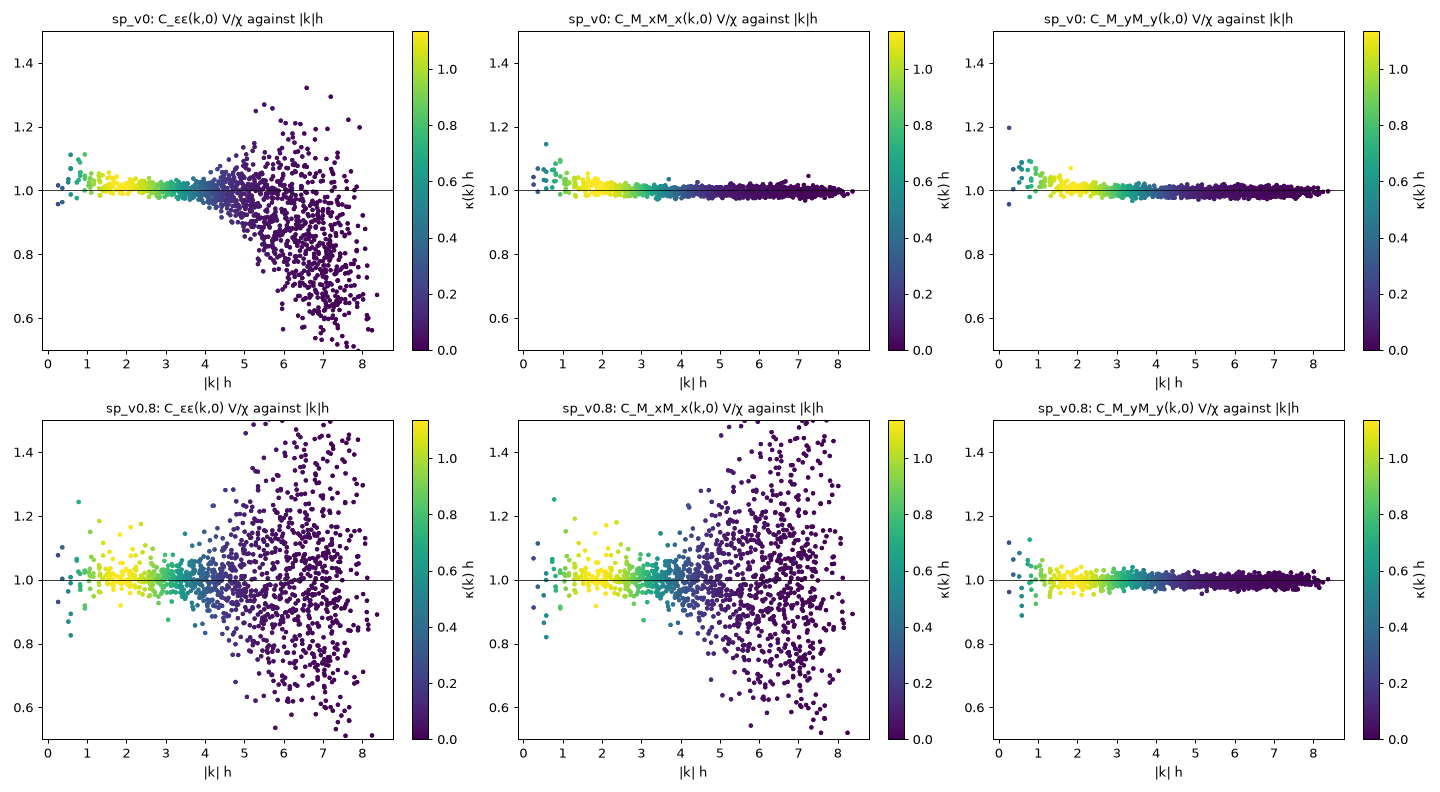
\includegraphics[width=\textwidth]{figs/grid_spectra_kh.png}
\caption{Equal-time spectra of every lattice mode, $C_{AA}(\bm k,0)V/\chi_{AA}$ against $|\bm k|h$, coloured by the lattice derivative
$\kappa(\bm k)h$; top $v_0=0$, bottom $v_0=0.8$; 16 runs each, $t=100$.}
\label{fig:gspkh}
\end{figure}
\begin{figure}[t]
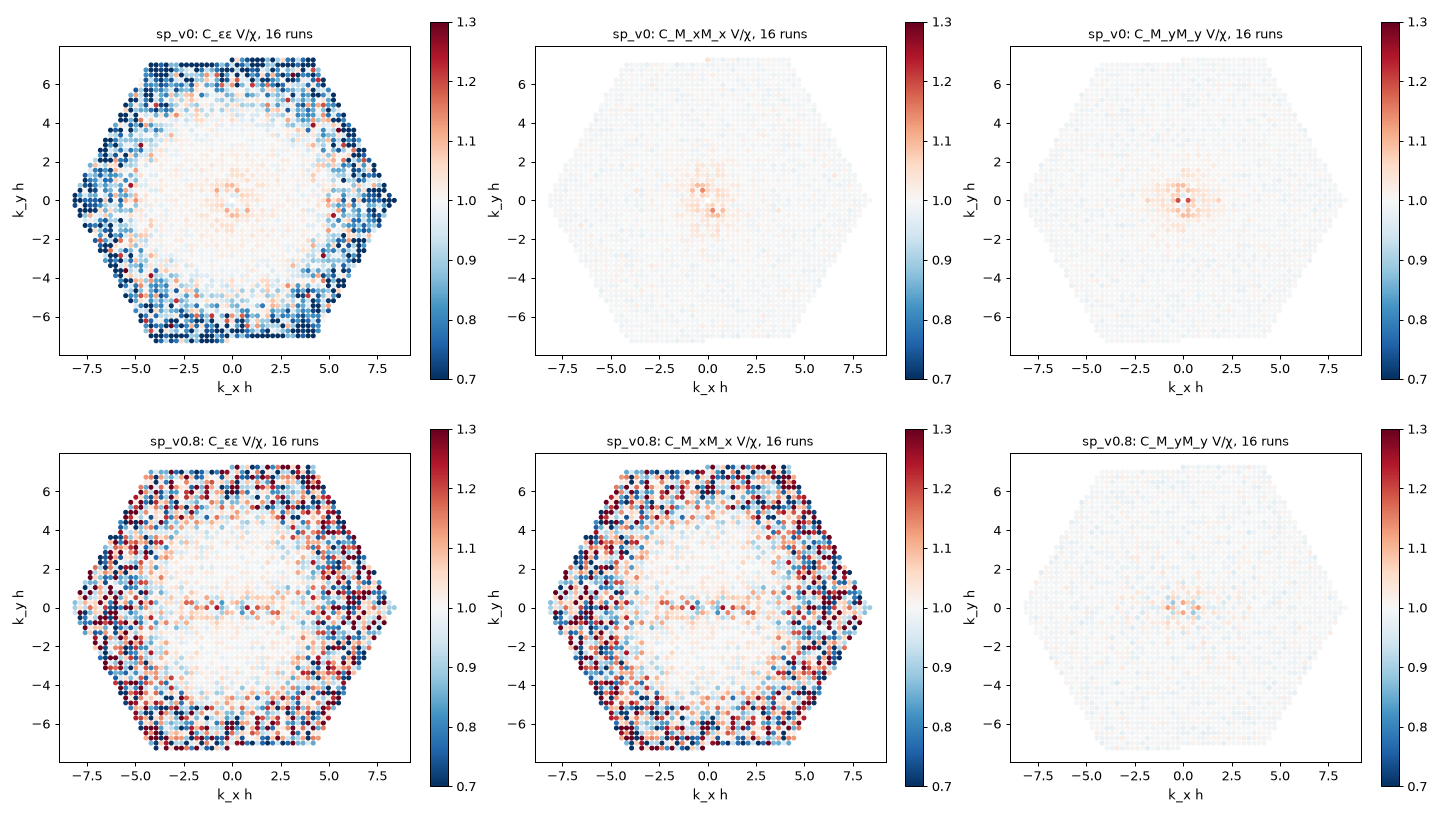
\includegraphics[width=\textwidth]{figs/grid_spectra_maps.png}
\caption{The same over the Brillouin zone ($k_xh$, $k_yh$; first-zone representatives): equipartition is white.}
\label{fig:gspmap}
\end{figure}
\begin{figure}[t]
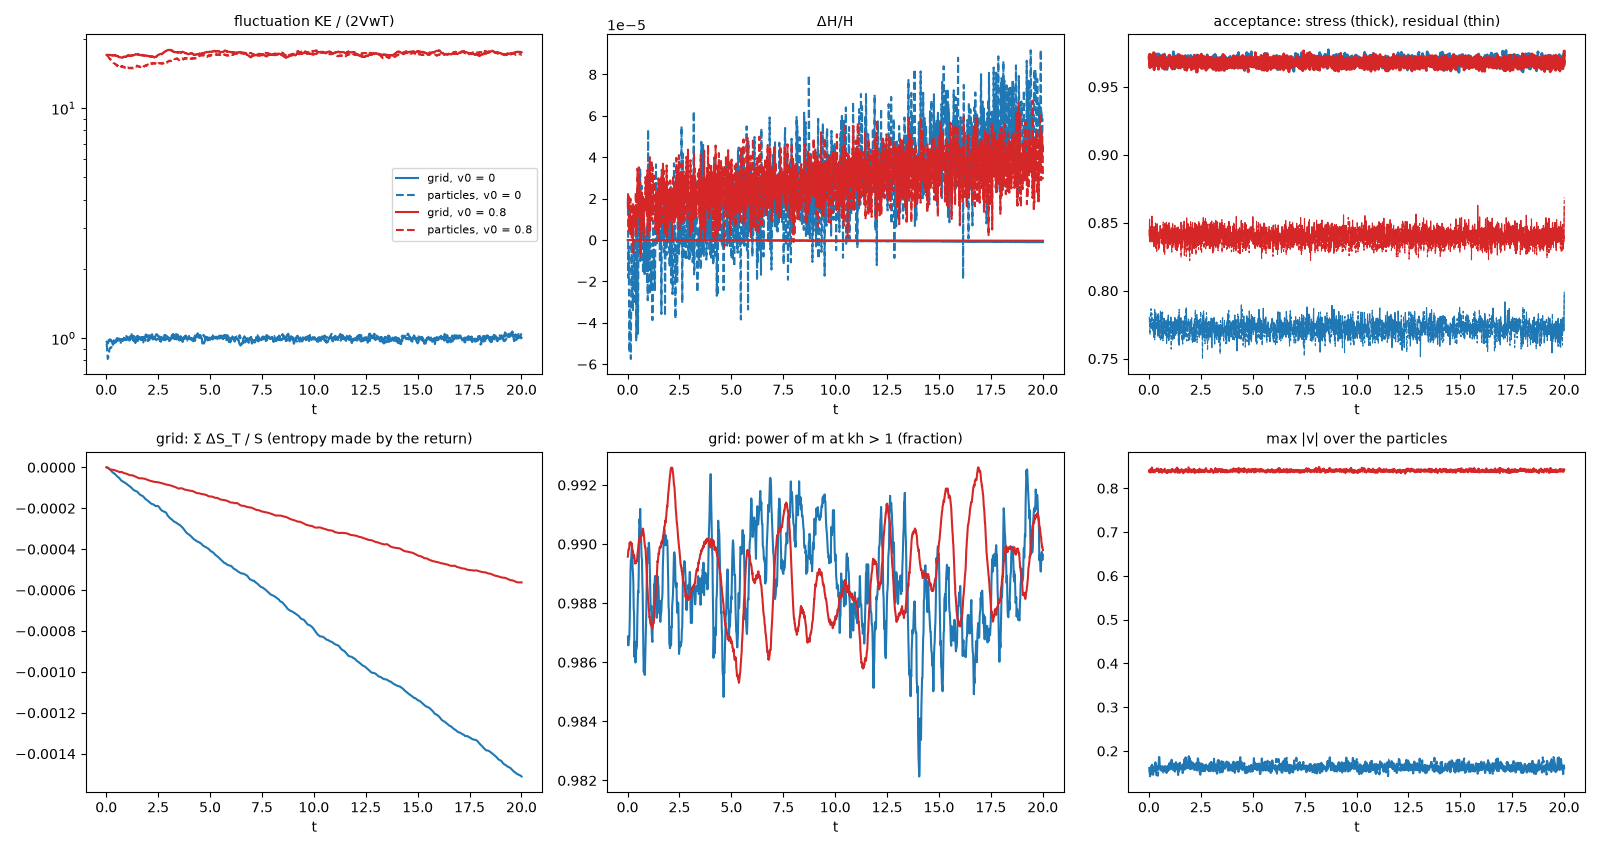
\includegraphics[width=\textwidth]{figs/grid_smoke.png}
\caption{Stochastic smoke test, $L=0.6$, 4 seeds each (mean): grid (solid) and particles (dashed), at rest
(blue) and at $v_0=0.8$ (red).  Fluctuation kinetic energy, $\Delta H/H$, acceptances, the entropy made
by the return, the fraction of the momentum power at $kh>1$, and the largest particle speed.}
\label{fig:gsmoke}
\end{figure}

\end{document}
